% THIS DOCUMENT IS FOLLOWS THE VOLERE TEMPLATE BY Suzanne Robertson and James Robertson
% ONLY THE SECTION HEADINGS ARE PROVIDED
%
% Initial draft from https://github.com/Dieblich/volere
%
% Risks are removed because they are covered by the Hazard Analysis

\documentclass[12pt]{article}

\usepackage{booktabs}
\usepackage{tabularx}
\usepackage{hyperref}
\usepackage{float}
\usepackage{graphicx}
\usepackage{tikz}
\usepackage{tikz-uml}
\usepackage{tabularray}
\usepackage{xcolor}

\hypersetup{
    bookmarks=true,         % show bookmarks bar?
      colorlinks=true,      % false: boxed links; true: colored links
    linkcolor=red,          % color of internal links (change box color with linkbordercolor)
    citecolor=green,        % color of links to bibliography
    filecolor=magenta,      % color of file links
    urlcolor=cyan           % color of external links
}

% ~~~~~~~ Glossary Content Goes Here ~~~~~~~

\usepackage[nonumberlist, nopostdot, nogroupskip]{glossaries}

% Define custom glossary types 
\newglossary[slg]{SWE}{swd}{swi}{Software Engineering Terms}
\newglossary[dlg]{domain}{dld}{dli}{Domain-Specific Research Terms}
\newglossary[glg]{general}{gld}{gli}{General Terms}

% Make glossaries
\makenoidxglossaries
 
% Software Engineering Related Technical Terms 

\newglossaryentry{api}{
    type=SWE,
    name={API}, 
    description={An interface or set of rules that allow different software systems to communicate with each other.}
}

\newglossaryentry{backend}{
    type=SWE,
    name={Backend}, 
    description={The server-side part of the system responsible for business logic, data processing, storage and retrieval.}
}

\newglossaryentry{frontend}{
    type=SWE,
    name={Frontend}, 
    description={The part of the system that the user interacts with (e.g. the website interface)}
}

\newglossaryentry{nlp}{
    type=SWE,
    name={Natural Language Processing (NLP)},
    description={A field of artificial intelligence that enables machine interpretation of human language.}
}

\newglossaryentry{database-schema}{
    type=SWE,
    name={Database Schema},
    description={The structure of a database, including tables, fields, and relationships}
}

\newglossaryentry{data-pipeline}{
    type=SWE,
    name={Data Pipeline},
    description={A sequence of data processing steps that transform raw inputs into usable outputs}
}

\newglossaryentry{metadata}{
    type=SWE,
    name={Metadata},
    description={Descriptive information about a dataset, such as trial number, injection count, or timestamps}
}

\newglossaryentry{llm}{
    type=SWE,
    name={Large Language Model (LLM)},
    description={An AI model capable of understanding and generating human-like language.}
}

\newglossaryentry{relational-database}{
    type=SWE,
    name={Relational Database},
    description={A database structured for relations among stored data, typically organized in tables with rows and columns}
}

\newglossaryentry{dbms}{
    type=SWE,
    name={Database Management System (DBMS)},
    description={Software that allows users to define, create, maintain, and control access to databases.}
}

\newglossaryentry{query}{
    type=SWE,
    name={Query},
    description={A structured request to retrieve or manipulate data from a database.}
}

\newglossaryentry{endpoint}{
    type=SWE,
    name={Endpoint},
    description={A specific URL or function in an API that allows access to a particular service or resource.}
}


\newglossaryentry{deployment}{
    type=SWE,
    name={Deployment},
    description={The process of making a software system available for use, including installing, configuring, and launching it in a target environment.}
}

%Domain Specific Research Terminology 

\newglossaryentry{ocd}{
    type=domain,
    name={Obsessive-Compulsive Disorder (OCD)},
    description={A psychiatric disorder characterized by intrusive thoughts and repetitive behaviors}
}

\newglossaryentry{rat-behavioral-trials}{
    type=domain,
    name={Rat Behavioral Trials},
    description={Controlled experiments recording rat movements and actions under specific conditions}
}

\newglossaryentry{spatial-temporal-data}{
    type=domain,
    name={Spatial-Temporal Data},
    description={Data that records both position (x, y coordinates) and time (t)}
}

\newglossaryentry{trajectory}{
    type=domain,
    name={Trajectory},
    description={The path taken by a rat during a trial, usually represented as a series of coordinates}
}

\newglossaryentry{behavioral-metrics}{
    type=domain,
    name={Behavioral Metrics},
    description={Quantitative measures of behavior, such as distance traveled or number of returns to a location}
}

\newglossaryentry{frdr}{
    type=domain,
    name={FRDR (Federated Research Data Repository)},
    description={The Canadian platform where the dataset is currently stored publicly}
}

%General Definitions

\newglossaryentry{open-source}{
    type=general,
    name={Open Source},
    description={Software whose source code is publicly available for use, modification, and distribution}
}

\newglossaryentry{user-interface}{
    type=general,
    name={User Interface (UI)},
    description={The visual and interactive elements that allow users to interact with a system}
}

\newglossaryentry{accessibility}{
    type=general,
    name={Accessibility},
    description={The design of systems so they can be used by people with diverse abilities and disabilities}
}

\newglossaryentry{usability}{
    type=general,
    name={Usability},
    description={The ease with which a user can learn and effectively interact with a system}
}

\glsaddallunused


\newcommand{\lips}{\textit{Insert your content here.}}

\input{../Comments}
\input{../Common}

\begin{document}

\title{Software Requirements Specification for \progname: subtitle describing software} 
\author{\authname}
\date{\today}
	
\maketitle

~\newpage

\pagenumbering{roman}

\tableofcontents

~\newpage

\section*{Revision History}

\begin{tabularx}{\textwidth}{p{3cm}p{2cm}X}
\toprule {\textbf{Date}} & {\textbf{Version}} & {\textbf{Notes}}\\
\midrule
Date 1 & 1.0 & Notes\\
Date 2 & 1.1 & Notes\\
\bottomrule
\end{tabularx}

~\\

~\newpage
\section{Purpose of the Project}
\subsection{User Business}

\par{The business of the user is to use the system to aid in the
creation and analysis of experiments relating to a large but fragmented data set
of \gls{rat-behavioral-trials} that investigate compulsive behaviour of rats and how they relate to various 
factors such as drug injections or brain legions. This data set is comprised of videos of rats
moving on a flat surface, files of their (x,y) coordinates and plots that show the \gls{trajectory} of these coordinates. Users may want to
extract a concise set of pre-existing data that can be applicable to
their hypothesis to streamline their workflow and avoid the necessity of carrying out trials.
Users may also want to use the system to provide analysis on the data set as a means of
further supplementing their academic work. This can include drawing \gls{behavioral-metrics} of the rats
based on various parameters (i.e. rate of compulsion based on injection type) or data visualizations
based similarly on compulsive behaviours as they relate to attributes of the rats.}


\subsection{Goals of the Project}

\par{The high-level goal of the project is to provide users in the field of behavioural sciences,
a unified and non-technical way of drawing from the vast amount of available data on \gls{ocd} rat trials
to aid in their academic work and experiments. This will be accomplished via the following sub-goals:}

\begin{itemize}
    \item Create a \gls{dbms} that provides \gls{query} access to the entirety of the data set of \gls{rat-behavioral-trials} as well as all \gls{metadata} associated with the data.
    \item Provide a UI that makes querying this data approachable to non-technical users by incorporating familiar and intuitive filtering and searching techniques
    (Attribute filters, Natural Language search bar). Further the UI must provide users with pre-generated query options that are likely to
    be useful for users that may not know where to start. This could include selecting all rat trials of a particular drug injection along with
    all saline control data.
    \item Provide an algorithm that can identify compulsive behaviour by looking at each rat trial
    and provide options for behavioural metrics and data visualizations based on various attributes that the user can extract 
    for their purposes.
\end{itemize}



\section{Stakeholders}

\subsection{Client}
\label{sec:2.1client}
\par{The clients for this project are Dr. Henry Szechtman and Dr. Anna Dvorkin-Gheva, two professors at McMaster University who are experts in
the fields of Psychiatry and Behavioural Neurosciences and Bioinformatics, respectively. They have worked extensively with these \gls{ocd} rat trials and
were responsible for generating and depositing this data in the \gls{frdr} repository where it currently is stored. Dr. Szechtman and Dr. Dvorkin-Gheva want
to drastically improve the availability of the vast data set they have created so that the trials they conducted can become useful to other students and academics in related fields. \\\\}




\par{Client Decisions}
\begin{itemize}
    \item User Interface (tools and organization of the data).
    \item The data that is accesible to the user.
    \item Goals of the project.
    \item Extensions and add ons in the project.
\end{itemize}



\begin{figure}[p]
    \centering
    \makebox[\textwidth][c]{%
        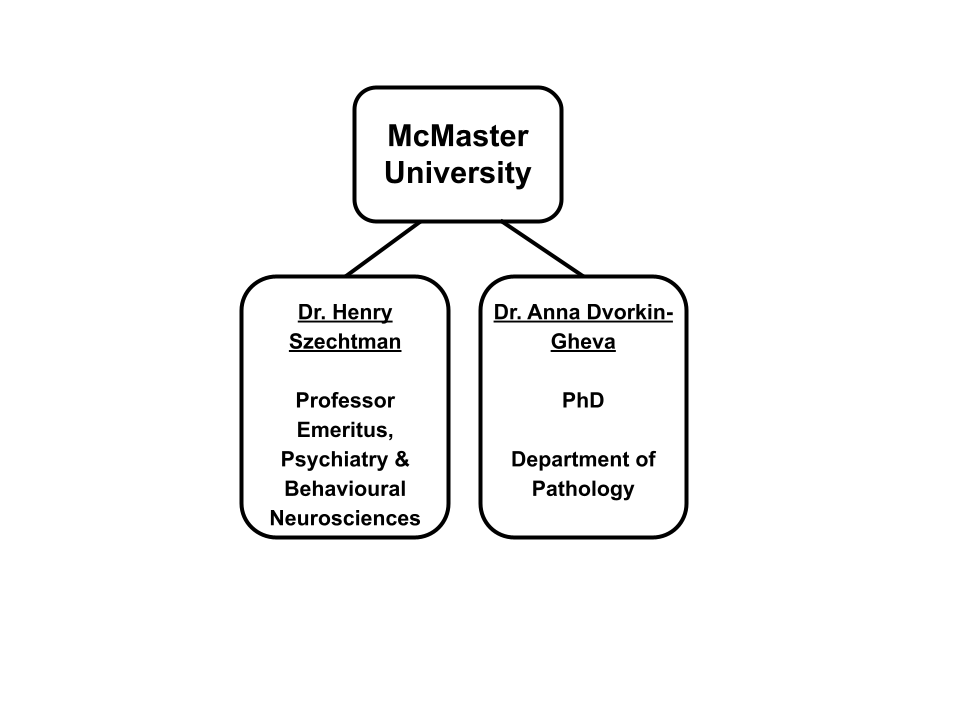
\includegraphics[width=1.1\textwidth]{2.1 Org Chart.png}%
    }
    \caption{Client Organizational Chart.}
    \label{fig:Client Org Chart}
\end{figure}

\begin{table}[H] 
    \centering
    \caption{Client and Customer Revision Dates}
    \label{tab:my_table} 

    \begin{tabular}{|l|c|} 
        \hline 
        Review Checkpoint & Date \\ 
        \hline 
        Revision 0 Design Demonstration  & Feb 2-13 2025 \\
        \hline 
        Final System Demonstration & Mar 23-29 2025 \\
        \hline 
    \end{tabular}
\end{table}
\par{Weekly meetings as well as external contact with professor will be done sporadically.}

\subsection{Customer}

\par{Since our application is intended to be \gls{open-source} and accessible to the public for free, our customers will simply be a group of end-users
of our application. Our end users will primarily involve behavioural neuroscience researchers like Dr. Henry Szechtman and Dr. Anna Dvorkin-Gheva, 
as well as graduate students and lab members, who will all benefit from the user-friendly and accessible functionality of the platform. 
Additionally we will have data scientists as customers, who will benefit from our application architecture and offered functionality for 
their purposes. Lastly, collaborating institutions and organizations from the open research community will be users of our application, 
since the application is intended to be free-use and accessible to all.\\\\}
\par{Revision Checkpoitns: See \hyperref[sec:2.1client]{2.1 Client}}


\subsection{Other Stakeholders}

\par{Other stakeholders for our project would be defined as any person or group of interest in the project outside the 
client and the customer. The first one would be our group, Gouda Engineers, as our task is to turn the project from the 
client/customer’s idea to a real product. We focus on creating documentation, building code, testing and deploying the 
software. Another stakeholder is our TA, Tiago de Moraes Machado, who is there to help our group along the way with our 
project by keeping us on track and providing feedback where it is needed. Lastly, our professor, Dr. Spencer Smith and our 
class, Capstone 4G06, would be the final stakeholders as they provide the guide and structure for building the project, 
knowledge on the topics for each step, and feedback where it is needed.}

\begin{figure}[H]
    \centering
    
\includegraphics[width=1\textwidth]{2.3 Other Stakeholders Chart.png}
    \caption{Stakeholder Chart.}
    \label{fig:stakeholder-chart}
\end{figure}

\subsection{Hands-On Users of the Project}
\label{sec:2.4handson}

The primary hands-on users of the Platform are those who will directly interact with the system for data access, analysis, and visualization. These include:

\begin{itemize}
    \item \textbf{Behavioral Neuroscientists:} Researchers who will query the dataset, visualize behavioral trajectories, and extract patterns for their studies.
    \item \textbf{Graduate and Undergraduate Students:} Students accessing subsets of the dataset for coursework, experiments, or learning purposes.
    \item \textbf{Data Scientists:} Users who programmatically analyze the data using Python or other tools, running algorithms and generating behavioral metrics.
    \item \textbf{Developers:} Individuals extending the platform or integrating it into custom workflows, running the system locally when needed.
\end{itemize}

These users will primarily interact with the system through the web interface for querying, filtering, using software tools for advanced analysis. 


\subsection{Personas}

Personas represent typical users of the system. They help in understanding user needs, goals, and interactions with the software. Each persona should include demographic information, technical expertise, motivations, and usage patterns. Personas are designed following the V.A.R.I.E.D. criteria (Vivid, Actionable, Realistic, Independent, Empathetic, Diverse) to ensure they are relatable and useful for design decisions.

\begin{itemize}
    \item \textbf{Persona Name:} Alex Johnson, Undergraduate Student
    \begin{itemize}
        \item \textbf{Role/Occupation:} Undergraduate student studying in the sciences.
        \item \textbf{Demographics:} 21 years old, male, undergraduate at McMaster University in Hamilton, Ontario, Canada.
        \item \textbf{Technical Expertise:} Basic knowledge in the sciences, familiar with query interfaces, moderate computer and data analysis skills.
        \item \textbf{Goals:} Search, filter, and download records from the database for coursework or research projects.
        \item \textbf{Tasks/Responsibilities:} Navigate the website, search and filter the database, access relevant datasets.
        \item \textbf{Pain Points:} Current data is unorganized, difficult to download, and hard to query.
        \item \textbf{Usage Scenario:} Accessing the platform during a lab session to analyze data and draw conclusions.
    \end{itemize}

    \item \textbf{Persona Name:} Jordan Lee, Developer
    \begin{itemize}
        \item \textbf{Role/Occupation:} Software developer or technical enthusiast.
        \item \textbf{Demographics:} 22 years old, non-binary, undergraduate-level knowledge, comfortable with computers and software, based in Toronto, Ontario, Canada.
        \item \textbf{Technical Expertise:} High technical skill in programming, database usage, and development tools.
        \item \textbf{Goals:} Extend system features or integrate the platform into custom workflows.
        \item \textbf{Tasks/Responsibilities:} DevOps, project management, software development, testing new features.
        \item \textbf{Pain Points:} Desired features may not yet be implemented; may need to work locally to customize functionality.
        \item \textbf{Usage Scenario:} Downloading the system to run locally and develop additional features or tools.
    \end{itemize}

    \item \textbf{Persona Name:} Dr. Maria Rodriguez, Advisors
    \begin{itemize}
        \item \textbf{Role/Occupation:} Experienced researchers or professors overseeing the project.
        \item \textbf{Demographics:} 45 years old, female, highly experienced in behavioral neuroscience, main stakeholders for the project, based in McMaster University.
        \item \textbf{Technical Expertise:} Advanced knowledge in the field and research methodologies.
        \item \textbf{Goals:} Ensure the system is scientifically accurate and usable for research.
        \item \textbf{Tasks/Responsibilities:} Provide guidance, make decisions on features, validate data integrity.
        \item \textbf{Pain Points:} Difficulty ensuring the data is accessible and reliable for all users.
        \item \textbf{Usage Scenario:} Reviewing the platform and verifying its usability for research purposes.
    \end{itemize}

    \item \textbf{Persona Name:} Sam Patel, Data Scientist
    \begin{itemize}
        \item \textbf{Role/Occupation:} Researcher or analyst focused on computational analysis.
        \item \textbf{Demographics:} 28 years old, male, graduate student or postdoctoral researcher with experience in data science, based in Vancouver, British Columbia, Canada.
        \item \textbf{Technical Expertise:} Proficient in Python, R, and statistical/machine learning tools.
        \item \textbf{Goals:} Analyze large-scale behavioral datasets, extract patterns, and generate insights.
        \item \textbf{Tasks/Responsibilities:} Run algorithms, process data, visualize results, integrate findings into research.
        \item \textbf{Pain Points:} Limited access to synchronized trajectory and video data; inefficient querying slows analysis.
        \item \textbf{Usage Scenario:} Programmatically accessing datasets to perform behavioral analysis and visualize results.
    \end{itemize}
\end{itemize}





\subsection{Priorities Assigned to Users}

\par{The key users for this project from the list in \hyperref[sec:2.4handson]{2.4 Hands-On Users of the Project} 
would be Behavioural Neuroscientists, Graduate and Undergraduate Students, and Developers as they are crucial 
to the long-term success of the project. The secondarcdy users would be data scientists as they will use the product 
but have little to no effect on long-term success.}

\subsection{User Participation}

\par{Estimated user participation time from \hyperref[sec:2.4handson]{2.4 Hands-On Users of the Project}:}
\begin{itemize}
    \item Behavioural Neuroscientists (1hr/week)
    \item Graduate and Undergraduate Students (1hr/week)
    \item Developers (10hr/week per developer)
\end{itemize}

\subsection{Maintenance Users and Service Technicians}

\par{Maintenance Users from \hyperref[sec:2.4handson]{2.4 Hands-On Users of the Project} :}
\begin{itemize}
    \item Developers
\end{itemize}

\par{Developers are hands-on users who must update, test, and maintain the project.}

\section{Mandated Constraints}
\subsection{Solution Constraints}

\begin{itemize}
    \item \textbf{SOL.C.1:} The system must be accessible via a web interface, with no installation required for end users.
    \item \textbf{SOL.C.2:} The system must interface with \\ \gls{frdr} to serve video files of the trials.
\end{itemize}

\subsection{Implementation Environment of the Current System}

\par{The OCD rat trial data set is currently hosted and accessible on the Federated Research Data Repository (FRDR), 
a Canadian national platform for research data management and sharing. The current environment has the following components:}

\begin{itemize}
    \item \textbf{User Environment}
    \begin{itemize}
        \item Users currently access datasets on FRDR through a standard web browser such as Google Chrome.
        \item No special software or hardware is needed, users can use any personal device such as their laptop or a mobile device.
    \end{itemize}
    \item \textbf{Data and Metadata Storage}
    \begin{itemize}
        \item The data set and its associated metadata are stored in FRDR's cloud-based infrastructure.
    \end{itemize}
    \item \textbf{Hosting and Maintenance}
    \begin{itemize}
        \item FRDR's cloud-based infrastructure is maintained by the Digital Research Alliance of Canada.
        \item FRDR's infrastructure incorporates redundant storage and regular data backups to ensure long-term data preservation and protection.
    \end{itemize}
    \item \textbf{Data Access and Technical Interfaces}
    \begin{itemize}
        \item Users can access and view the data set through FRDR's web portal.
        \item Data accessed through the web portal can be downloaded through links on the web page.
        \item FRDR also exposes an API specifically for data set querying and retrieval.
    \end{itemize}
\end{itemize}

\par{The following diagram is a rough outline of the form of the current system:}

\begin{figure}[H]
    \centering
    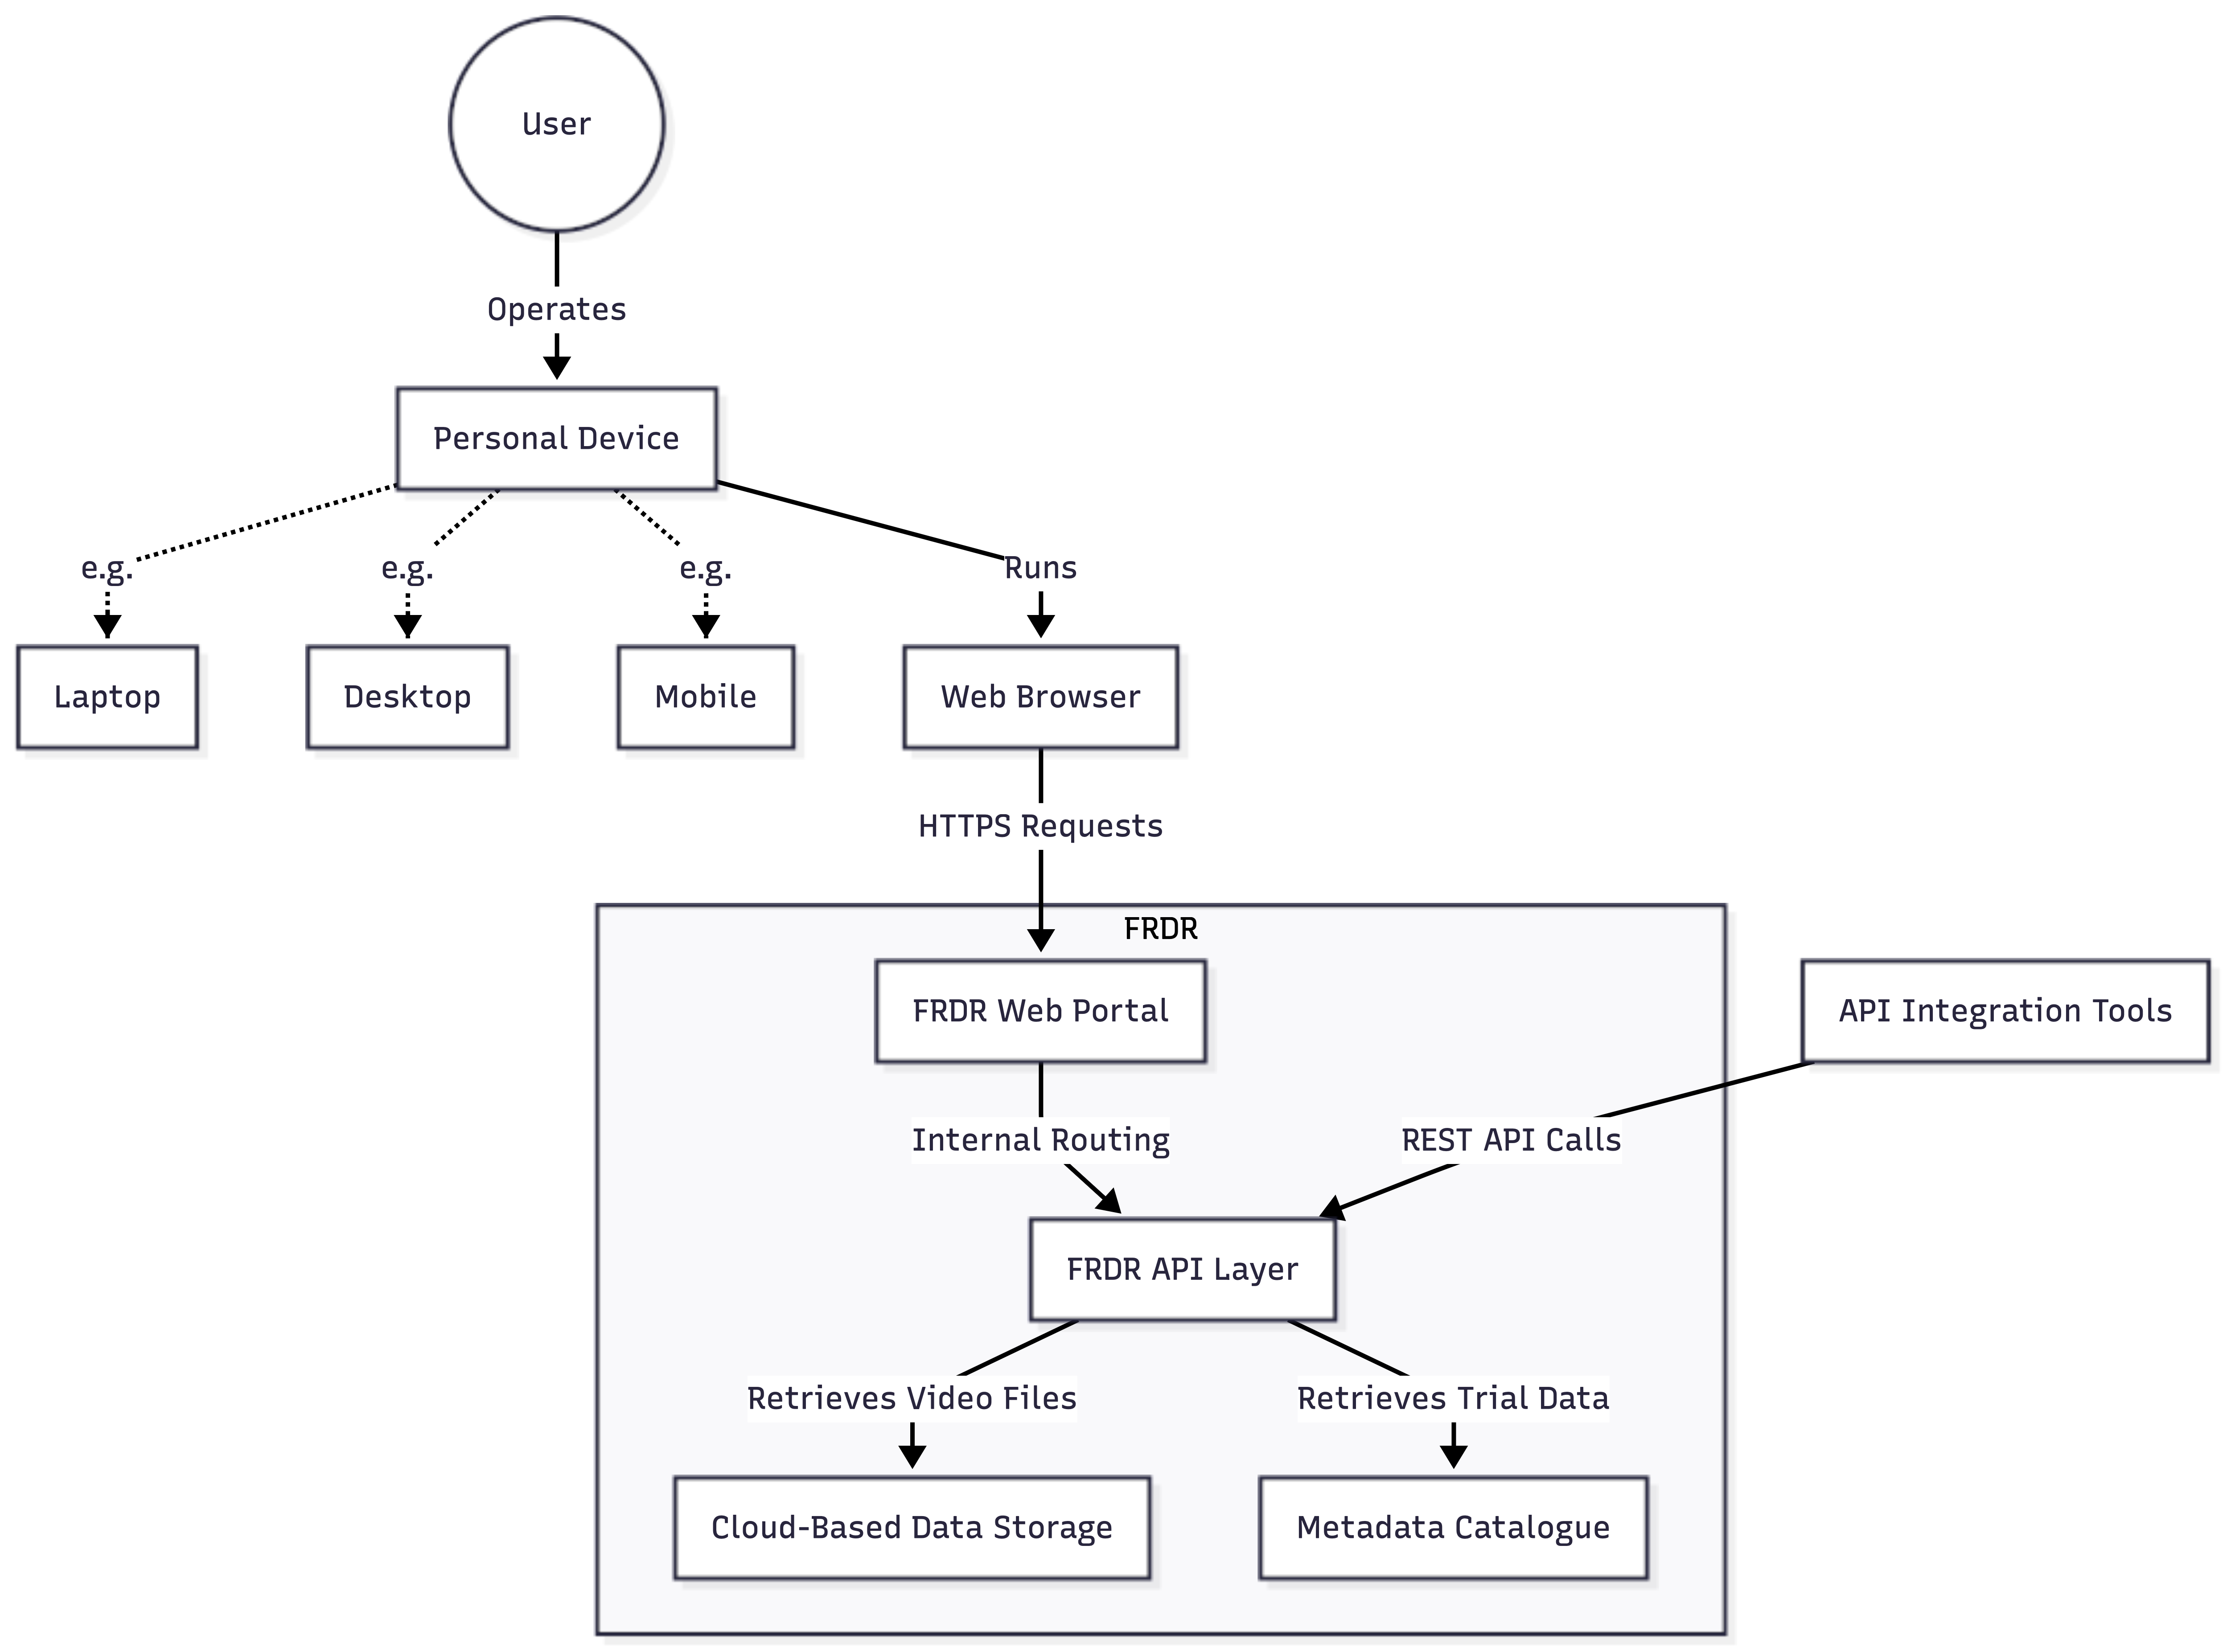
\includegraphics[width=1\textwidth]{3.2 Current System (Form) Diagram.png}
    \caption{Current System (Form) Diagram.}
    \label{fig:currentSysForm}
\end{figure}

\subsection{Partner or Collaborative Applications}

\begin{tabular}{|m{5cm}|m{10cm}|}
    \hline
    Collaborative System & System Overview \\
    \hline
    FRDR Repository & The Federated Research Data Repository is a 'bilingual bilingual publishing 
    platform for sharing and 
    preserving Canadian research data. 
    It is a curated, general-purpose repository, 
    custom built for large datasets.' This is where the data set of the rat trials is physically located
    and is dispersed across 29 independent datasets. Our system will provide a unified database schema but will
    pull data from this repository.\\
    \hline
    ratbat.mcmaster.ca & While not a directly collaborative system, this is a system made by a previous years' capstone
    team to address the same problem that our system seeks to. It will be a collaborative system in the sense that ir provides
    a reference of potential ways to approach our solution, ideas that work well and can be carried forward
    and providing visibility to shortcomings of the system will help us to avoid repeating mistakes. \\
    \hline
\end{tabular}

\subsection{Off-the-Shelf Software}

\begin{itemize}
    \item The system shall make use of the FRDR API in order to fetch the relevant data from the data set as we will not be hosting a seperate database to physically store the data for our system
    \item In the case of implementing natural language processing, an Off-the-Shelf LLM will be used to accomplish this (In other words we will not be writing our own LLM model for this purpose).
    Note that this model may need to be trained to provide results that are acceptable for our purposes.
\end{itemize}

\subsection{Anticipated Workplace Environment}

The anticipated workplace environment for the software system includes:

\begin{itemize}
    \item The workspace is defined as the computer environment where the software will operate.
    \item The system is expected to be used primarily on standard desktop or laptop computers with modern operating systems such as Windows, macOS, or Linux.
    \item Users will access the system through web browsers (e.g., Chrome, Edge, Safari) or dedicated client applications, depending on the software configuration.
    \item The system may require external software installed to run locally, such as Docker and Kubernetes.
\end{itemize}

\subsection{Schedule Constraints}

\par{Due to the nature of the capstone course, the scheduling constraints
map directly to dates in which major deliverable related to the project are due in the capstone course.
They are laid out below:}

\begin{tabular}{|m{5cm}|m{10cm}|}
    \hline
    Project Milestone & Scheduling Constraint \\
    \hline
    Software Requirements Specification \textbf{(SCH.C.1)} & Oct 6 2025 \\
    \hline
    Verification and Validation Plan \textbf{(SCH.C.2)} & Oct 27 2025\\
    \hline
    Design Document Revision -1 \textbf{(SCH.C.3)} & Nov 10 2025\\
    \hline
    Proof of Concept Demonstration \textbf{(SCH.C.4)} & Nov 17-28 2025\\
    \hline
    Design Documentation Revision 0 \textbf{(SCH.C.5)} & Jan 19 2025\\
    \hline
    Revision 0 Design Demonstration \textbf{(SCH.C.6)} & Feb 2-13 2025\\
    \hline
    Verification and Validation Report \textbf{(SCH.C.7)}  & Mar 9 2025\\
    \hline
    Extras (Performance Report + User Manual) \textbf{(SCH.C.8)} & Mar 9 2025\\
    \hline
    Final System Demonstration \textbf{(SCH.C.9)} & Mar 23-29 2025\\
    \hline
    Final Documentation \textbf{(SCH.C.10)} & April 6 2025\\
    \hline
\end{tabular}




\subsection{Budget Constraints}

\par{\textbf{BUD.C.1:} There is very limited budget available for this project. The department of Computing and Software at McMaster University 
will provide \$125 CAD for approved expenses. Outside of that funding, we are asked not to exceed spending of \$500 CAD
culmulatively as a team. Thus, the total budget constraints for this project are \$500 CAD in total and \$375 of our team's personal funding.}

\subsection{Enterprise Constraints}

\begin{itemize}
    \item \textbf{ENT.C.1:} The project must be designed such that it can be maintained by future students, or researchers after the conclusion of the capstone project. 
    \item \textbf{ENT.C.2:} All project documentation must be archived in a public repository to ensure accessibility for future use and extension. 
\end{itemize}

\section{Naming Conventions and Terminology}
\subsection{Glossary of All Terms, Including Acronyms, Used by Stakeholders
involved in the Project}

\printnoidxglossary[type=SWE, title={Software Engineering Terms}]
\printnoidxglossary[type=domain, title={Domain-Specific Research Terms}]
\printnoidxglossary[type=general, title={General Terms}]



\section{Relevant Facts And Assumptions}
\subsection{Relevant Facts}

\begin{itemize}
    \item The entirety of the data set that is being worked with is available in the FRDR repository
    but is fragmented into 29 independent dats sets. 29 being the number of studies written that required relevant
    rat trials to be performed.
    \item The culmination of all the relevant data for this project is 11 terabytes and contains nearly 60,000 data objects with
    20,000 hours of video files alone.
    \item Every data object has many metadata annotations (or attributes) associated within them. In the current data hosting
    implementation on the FRDR, these are all contained in a README file that is stored in the root directory of each dataset.
    This README file has a row for each data object in the dataset and columns for each attribute.
\end{itemize}

\subsection{Business Rules}

    \par{This system does not exist within a traditional business environment and is
    rather in the realm of academia. As a result, there are no specific business rules that shape
    the requirements, the system acts as a tool in academic pursuits. Additionally, any business rules
    related to protection of information do not apply as all data being used is publicly available to
    the general public already. }

\subsection{Assumptions}

The following assumptions form the foundation of this system specification. Each assumption includes its explicit scope boundary, detailing what the system is and is not responsible for:

\begin{itemize}
    \item \textbf{ASSUMPTION.1 --- FRDR Availability:} We assume that the Federated Research Data Repository (FRDR) will maintain data availability and accessibility for the duration of this project's lifecycle. \textit{System Boundary: The system is NOT responsible for FRDR outages, data corruption at FRDR, or FRDR service discontinuation. Users experiencing FRDR unavailability will receive informative error messages but the system cannot guarantee data access if FRDR is offline.}
    
    \item \textbf{ASSUMPTION.2 --- External Data Storage Model:} We assume the system will not need to physically store copies of the behavioral trial data locally, and can depend entirely on \\gls{frdr} as the authoritative data source. \textit{System Boundary: The system is NOT designed for local data caching/replication. All query operations assume network access to FRDR. Offline operation is not supported for data queries, though the web interface may function in a limited read-only state.}
    
    \item \textbf{ASSUMPTION.3 --- FRDR API Availability:} We assume the FRDR repository will provide and maintain API access to dataset metadata and file objects. \textit{System Boundary: The system depends on FRDR API contract stability. If the FRDR API changes or is deprecated, system functionality would require architectural redesign. The system is NOT responsible for negotiating API changes with FRDR.}
    
    \item \textbf{ASSUMPTION.4 --- FRDR API Performance:} We assume the FRDR API will deliver query results with latency that enables our 2-second response time target (SAL.R.1). \textit{System Boundary: System performance is bounded by FRDR response times. If FRDR latency exceeds 1.5 seconds, the 2-second requirement cannot be met. The system is NOT responsible for optimizing FRDR infrastructure.}
    
    \item \textbf{ASSUMPTION.5 --- Machine Learning Model Availability:} We assume suitable pre-trained or trainable machine learning models will be available for natural language query processing and behavioral categorization. \textit{System Boundary: The system is NOT responsible for developing custom AI models from scratch. Implementation assumes third-party models (e.g., OpenAI API, Google Vertex AI) remain available and functional. Model accuracy failures are beyond system scope.}
    
    \item \textbf{ASSUMPTION.6 --- Client Platform Independence:} We assume web API requests are platform-independent and that users can access the system from any modern browser without special local software installation. \textit{System Boundary: The system requires a modern web browser with JavaScript/HTML5 support. Users on legacy systems, isolated networks, or with restrictive security policies may experience reduced functionality. The system is NOT designed for embedded or specialized hardware.}
    
    \item \textbf{ASSUMPTION.7 --- Research Data Stability:} We assume the underlying OCD rat trial data will remain scientifically valid and that no systematic errors in the source data will require widespread correction during the project lifecycle. \textit{System Boundary: The system assumes data integrity at FRDR. If systematic data errors are discovered, the system provides query capability but cannot retroactively correct erroneous results already downloaded by users.}
    
    \item \textbf{ASSUMPTION.8 --- PostgreSQL Viability:} We assume PostgreSQL will remain a viable, well-maintained relational database solution for the project's 5-year maintenance window. \textit{System Boundary: The system is NOT designed for migration to alternative database technologies (e.g., NoSQL, blockchain). Architectural refactoring would be required if PostgreSQL needs replacement.}
    
    \item \textbf{ASSUMPTION.9 --- Technology Ecosystem Stability:} We assume React, TypeScript, FastAPI, and Python ecosystem components will remain stable, well-supported technologies throughout the project lifecycle. \textit{System Boundary: The system may require dependency updates and patches but is NOT designed to accommodate wholesale technology replacements (e.g., switching from React to Vue, or Python to Go).}
    
    \item \textbf{ASSUMPTION.10 --- Maintenance Team Availability:} We assume future development teams will have sufficient technical documentation and code clarity to maintain and extend the system beyond the initial capstone project term. \textit{System Boundary: The system depends on documentation quality (Design Document, User Manual, inline code comments) to remain maintainable. If documentation becomes outdated or lost, future maintenance becomes significantly more costly.}
    
    \item \textbf{ASSUMPTION.11 --- Internet Connectivity:} We assume all end users have reliable internet connectivity and can access web-hosted services at latencies below 100ms. \textit{System Boundary: Users on high-latency connections (satellite, remote regions) may experience degraded performance. The system is NOT optimized for low-bandwidth or intermittent connectivity scenarios.}
    
    \item \textbf{ASSUMPTION.12 --- Dataset Scope Stability:} We assume the OCD rat behavioral trial dataset will not expand beyond the current 11 TB capacity during the 5-year operational lifespan. \textit{System Boundary: The database and infrastructure are sized for 11 TB. Significant dataset expansion would require infrastructure scaling. The system is NOT designed for dynamic, unbounded data growth.}
\end{itemize}


\section{The Scope of the Work}
\subsection{The Current Situation}

\par{ The current situation currently revolves the \gls{frdr} as a means
of depositing and extracting data. Dr. Henry Szechtman and Dr. Anna Dvorkin-Gheva have
deposited the relevant data related to their work into this repository. The repository
has this data seperated into 29 distinct datasets, based on the specific study the data relates to.
Additionally, there is a large amount of metadata that is not well related to the data objects it describes
(it is stored in a readme file in each dataset which is seperate from the actual data objects). As a result, while
users are able to access all of the available data, it is very fragmented, nearly impossible to filter and search
effectively and hard to leverage for any specific research purposes. \newline\newline

Additionally, the project from last year, RatBat \cite{GitHub_RatBAT}, is also pulling from the \gls{frdr}
dataset using its provided API. Please see below of a graphical layout of the current situation.\newline\newline

\indent Note that each arrow simply indicates an exchange of information from the system to some cooperating component or vice versa.}

\begin{figure}[H]
    \centering
    \includegraphics[width=0.8\textwidth]{6.1 Current Situation.png}
    \caption{The Current Situation}
    \label{fig:current-situation}
\end{figure}


\subsection{The Context of the Work}

\begin{figure}[H]
    \centering
    \includegraphics[width=0.8\textwidth]{6.2 Context of the Work.png}
    \caption{The Context of the Work}
    \label{fig:context-work}
\end{figure}

\subsection{Work Partitioning}

The work is divided into the following components to ensure clarity, manageability, and efficient development:

\begin{itemize}
    \item \textbf{Database Design and Backend Development:} 
        \begin{itemize}
            \item Design a robust PostgreSQL database schema for behavioral data, metadata, video files, and research files.
            \item Implement REST API endpoints for data querying, filtering, and downloading.
            \item Create efficient indexing and file management systems for large-scale spatial-temporal data and video content.
        \end{itemize}
        
    \item \textbf{Interactive Web Interface:} 
        \begin{itemize}
            \item Build a React-based frontend with search and filtering capabilities.
            \item Implement natural language querying for intuitive exploration of behavioral datasets.
            \item Develop data visualization tools for plotting trajectories and behavioral metrics.
            \item Integrate synchronized video playback with trajectory data.
            \item Design user-friendly interfaces accessible to researchers without programming experience.
        \end{itemize}
        
    \item \textbf{Data Processing Pipeline:} 
        \begin{itemize}
            \item Develop Python tools to process spatial-temporal coordinate data into meaningful behavioral measures.
            \item Implement algorithms to detect key behavioral patterns (e.g., home-base behavior, checking routes, exploration metrics).
            \item Create automated analysis workflows for common research tasks.
            \item Ensure the architecture is extensible for future video analysis capabilities.
        \end{itemize}
        
    \item \textbf{NLP Integration:} 
        \begin{itemize}
            \item Integrate language model APIs to support natural language queries.
            \item Implement keyword dictionaries for common domain terms (e.g., "compulsive behavior", "injection type") to improve query parsing accuracy.
            \item Add caching for frequent natural language queries to reduce processing time and LLM API costs.
            \item Develop detailed prompt engineering with domain-specific rulesets and examples to offset LLM limitations.
            \item Provide fallback to structured filters if NLP parsing fails.
        \end{itemize}
        
    \item \textbf{Deployment and DevOps:} 
        \begin{itemize}
            \item Deploy the platform for online access with reliability and scalability.
            \item Implement caching, backup, and security measures.
        \end{itemize}
        
    \item \textbf{Documentation and Tutorials:} 
        \begin{itemize}
            \item Prepare user manuals, tutorials, and technical documentation for researchers.
            \item Provide guidelines for extending and maintaining the platform.
        \end{itemize}
\end{itemize}



\subsection{Specifying a Business Use Case (BUC)}

\par{ Shown below is the Business Use Case diagram for our system. The
events that can be accessed by an actor are the business use cases and rest of the
diagram objects represent business events.\newline\newline
\indent Note that each arrow represents an "includes" relationship which is a top-down approach
to the use case with the most high level event (the use case) at the beginning and every subsequent step
being more granular. i.e. every subsequent step of the business event must be performed for the initial one to be completed. }


\begin{figure}[p]
    \centering
    \makebox[\textwidth][c]{%
        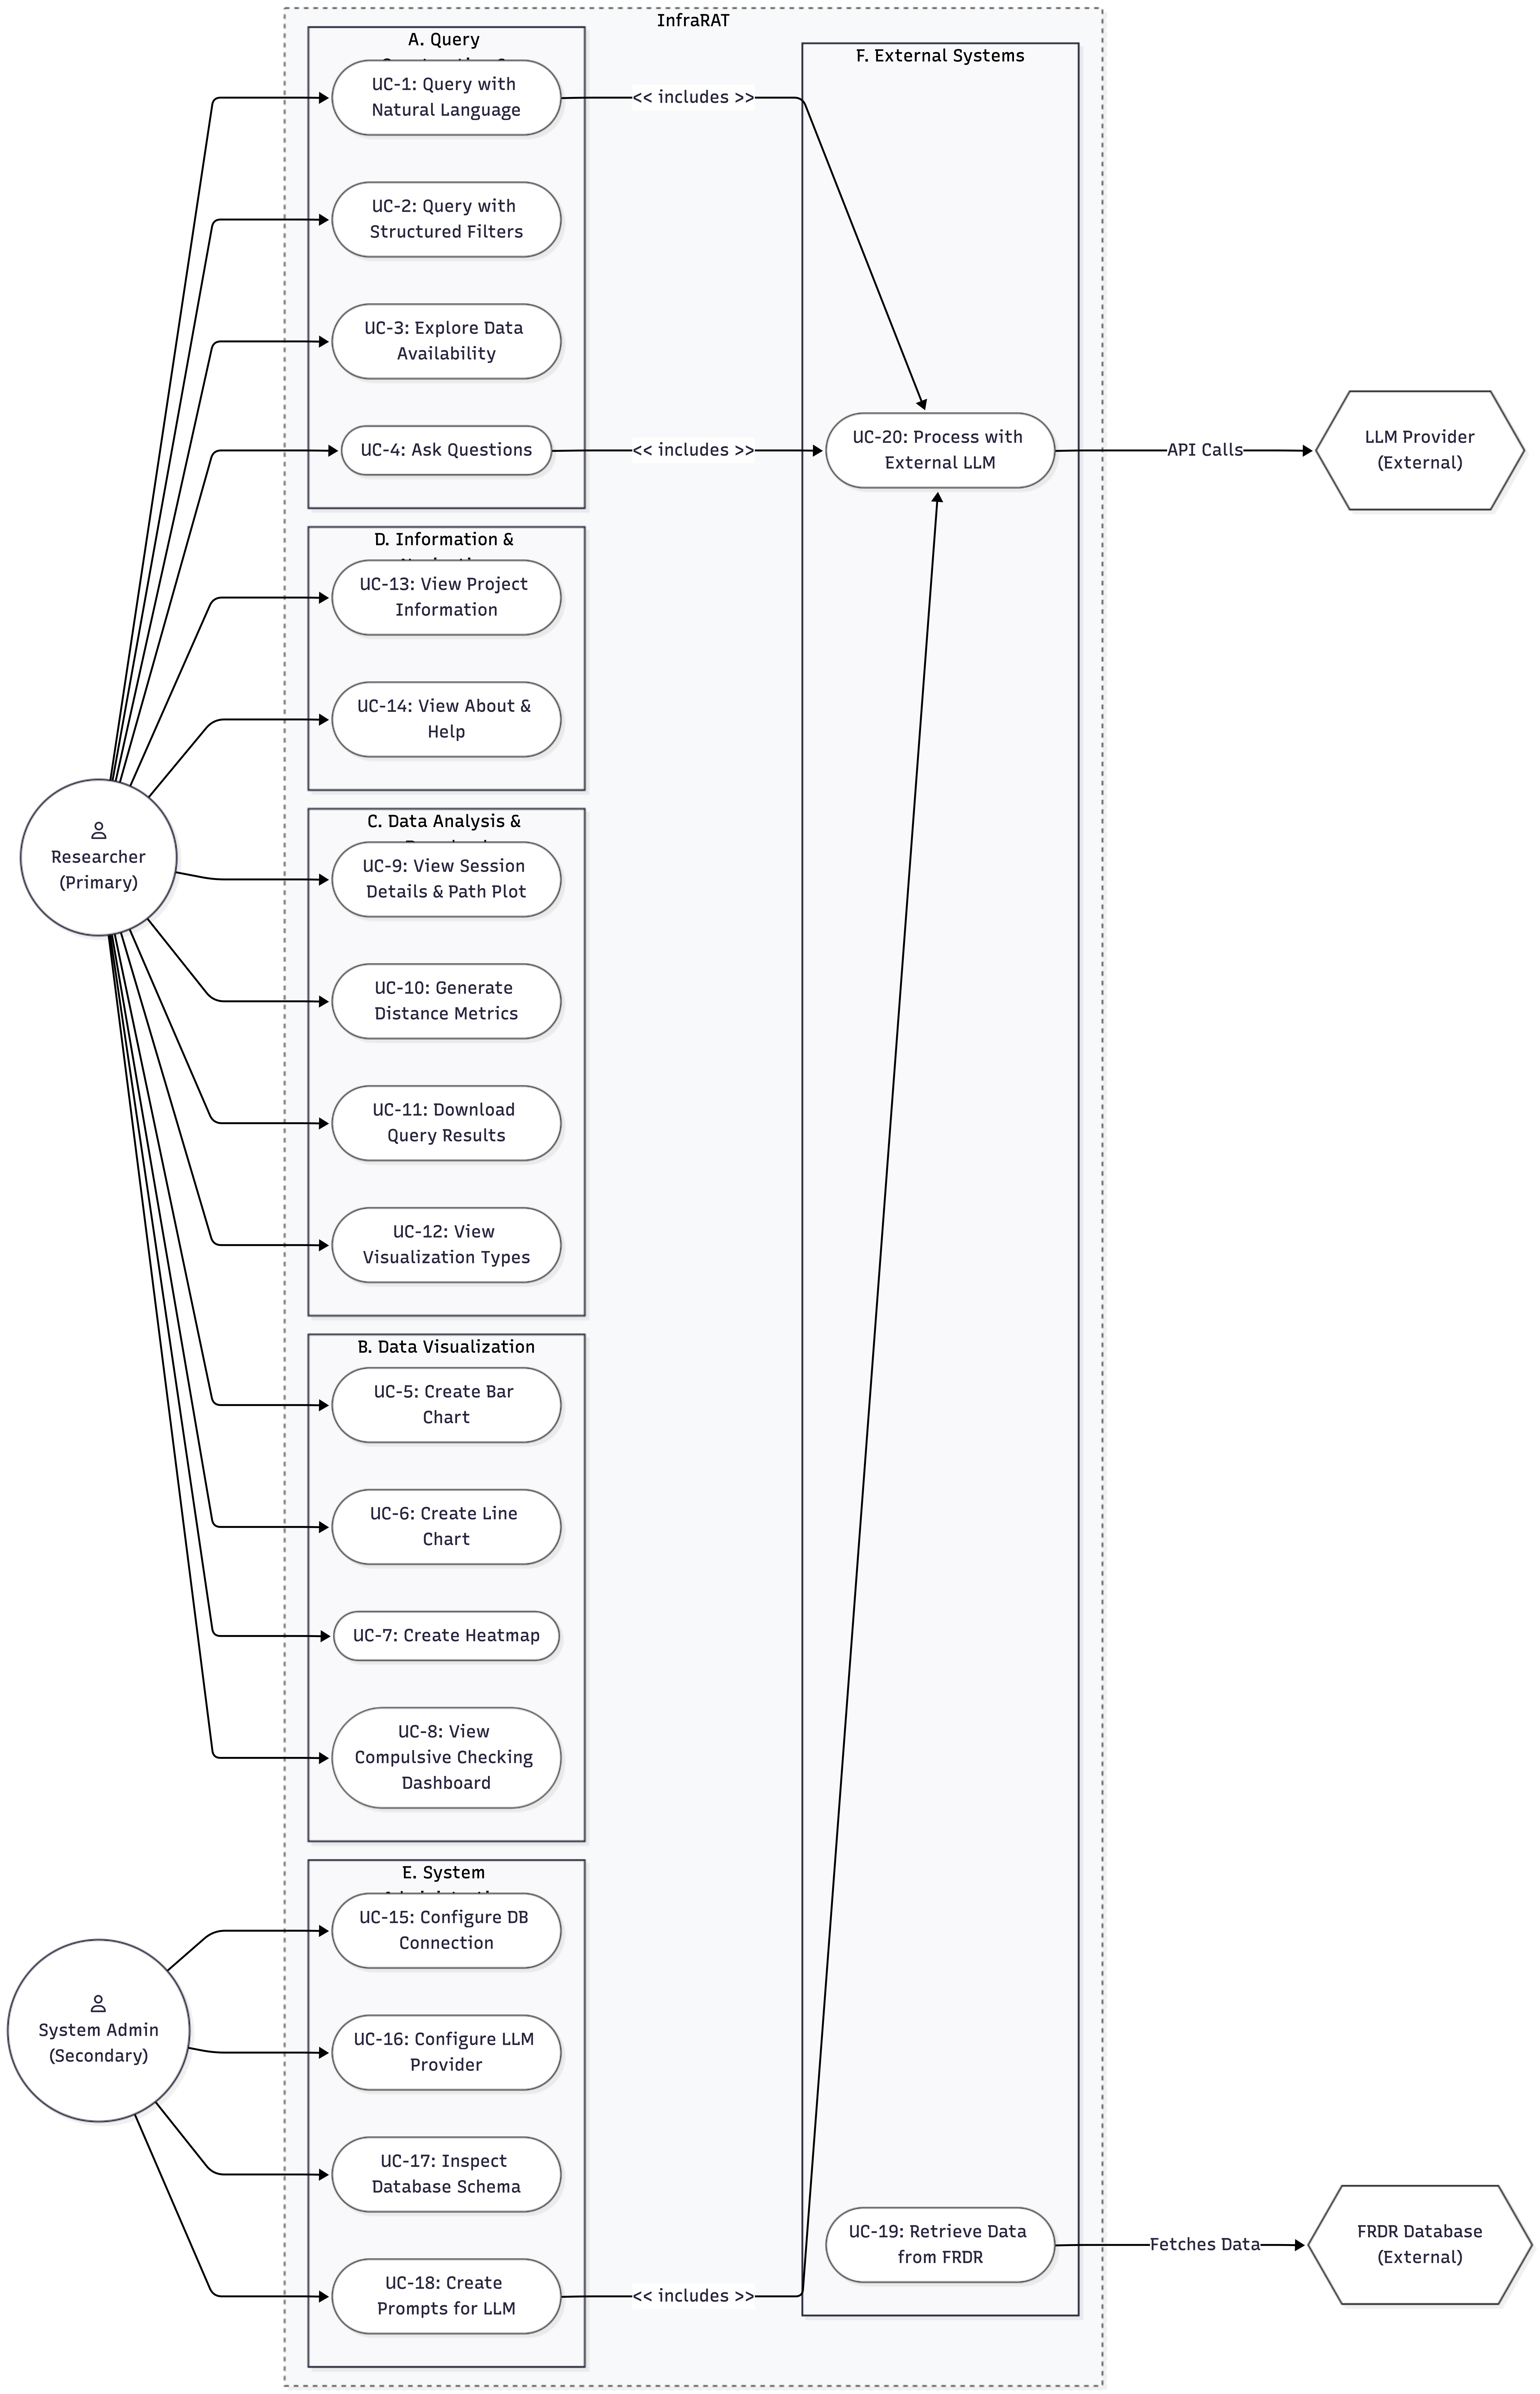
\includegraphics[width=1\textwidth]{6.4 Use Case Diagram.png}%
    }
    \caption{Use Case Diagram}
    \label{fig:UseCaseDiagram}
\end{figure}

\begin{table}[H]
\begin{tabular}{|m{2.5cm}|m{2cm}|m{3.0cm}|m{3.0cm}|m{2.5cm}|m{2.5cm}|}
\hline
\textbf{Use Case} & \textbf{Actors} & \textbf{Description} & \textbf{Outcome} & \textbf{Functional Requirement}\\ 
\hline
BUC1: Get Result Set & Researcher & Query dataset & Filtered dataset returned & \hyperref[req:func.r.1]{FUNC.R.1}, \hyperref[req:func.r.2]{FUNC.R.2}, \hyperref[req:func.r.3]{FUNC.R.3}\\
\hline
BUC2: Download Data & Researcher & Download trials & Files downloaded  & \hyperref[req:func.r.6]{FUNC.R.6} \\
\hline
BUC3: Get Data Visualizations & Researcher & Generate visualizations based on a requested data set & Graphical visualizations related to relevant dataset & \hyperref[req:func.r.5]{FUNC.R.5}\\
\hline
BUC4: Get Behavioural Metrics & Researcher & Generate statistical metrics of rat behaviour & Statistical breakdown of behavioural metrics in relevant dataset & \hyperref[req:func.r.4]{FUNC.R.4}\\
\hline
BUC5: Deposit Data & Dr. Henry Szechtman/Dr. Anna Dvorkin & Deposit New Data into FRDR & New data becomes available & Handled By Methods outside of System Scope \\
\hline
\end{tabular}
\caption{Business Use Case Table}
\end{table}


\section{Business Data Model and Data Dictionary}
\subsection{Business Data Model}

The Business Data Model in Figure \ref{fig:myimage} presents the major entities and relationships that describe how the system, the research users, and the underlying experimental data are structured. The model is centered on the Trial entity, which captures a single behavioral session and links the trial to the subject rat, the associated behavioral observations, the experimental conditions, and the supporting metadata. It also shows the human stakeholders involved in the project, including the Researcher, the Project Supervisor, and the Developer, to illustrate how user roles relate to the system and its data.

The key diagram elements are:
\begin{itemize}
    \item \textbf{Researcher:} A primary system user who queries data, reviews trial results, and interprets behavior measures.
    \item \textbf{Project Supervisor:} The academic or research supervisor overseeing the project, connected to researcher and developer roles to reflect governance and oversight.
    \item \textbf{Developer:} The team member responsible for building and maintaining the system.
    \item \textbf{FRDR Repository:} The external research data source where trial records are stored and from which the system ingest or references experimental datasets.
    \item \textbf{Trial:} The central business object representing a single experiment session, including identifiers, timing, injection details, and notes.
    \item \textbf{Rat:} The animal subject associated with each trial, with attributes such as weight, sex, age, and strain.
    \item \textbf{Condition:} The experimental condition or treatment applied during a trial, including severity, duration, and notes.
    \item \textbf{Behavior:} Observed behaviors recorded for each trial, including descriptions, timestamps, and intensity.
    \item \textbf{Metadata:} Supporting files and descriptive information for each trial, including file type, size, keys, and values.
\end{itemize}

\begin{figure}[H]
\begin{center}
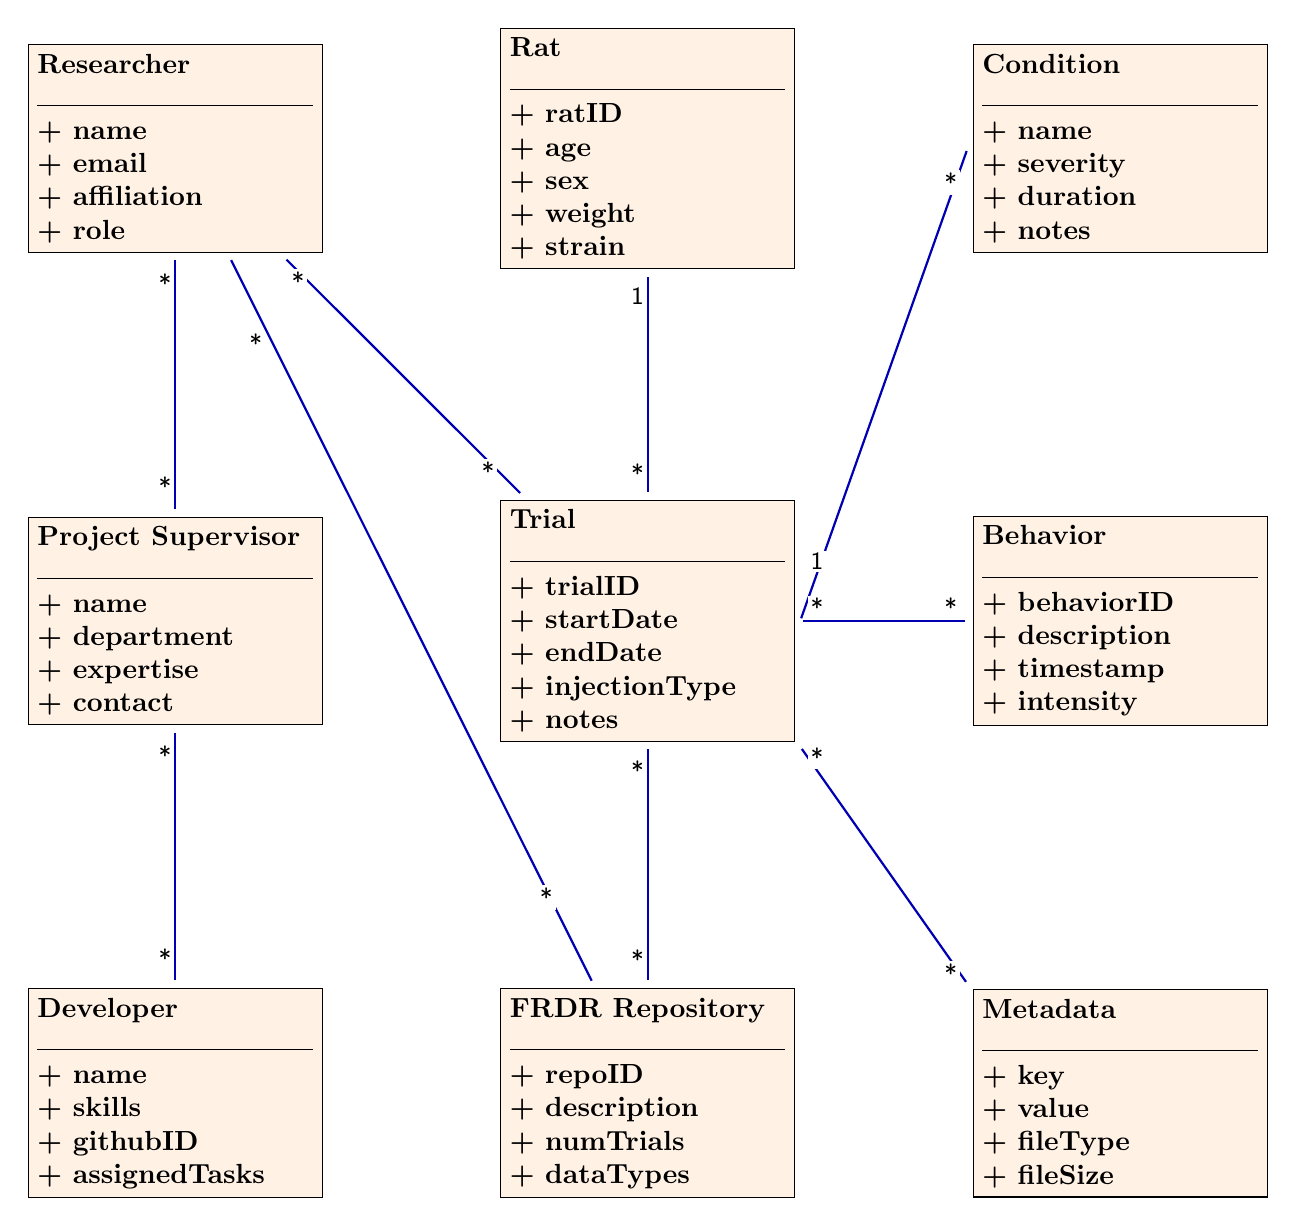
\begin{tikzpicture}[
    auto,
    umlclass/.style={
        rectangle,
        draw,
        fill=orange!10,
        text width=3.5cm,
        minimum height=1cm,
        align=left,
        font=\bfseries,
        outer sep=2pt,
        node distance=4cm
    },
    umlrelationship/.style={
        -,-,
        line width=0.8pt,
        draw=blue!70!black,
        shorten >=1pt, shorten <=1pt
    },
    multiplicity/.style={
        font=\sffamily\small,
        fill=white,
        inner sep=1pt
    },
    every node/.style={font=\sffamily\small}
]

% Classes with more attributes separated by line
\node[umlclass] (Researcher) at (0,12) {Researcher\\ \rule{\linewidth}{0.4pt}\\ + name\\ + email\\ + affiliation\\ + role};
\node[umlclass] (Supervisor) at (0,6) {Project Supervisor\\ \rule{\linewidth}{0.4pt}\\ + name\\ + department\\ + expertise\\ + contact};
\node[umlclass] (Developer) at (0,0) {Developer\\ \rule{\linewidth}{0.4pt}\\ + name\\ + skills\\ + githubID\\ + assignedTasks};

\node[umlclass] (FRDR) at (6,0) {FRDR Repository\\ \rule{\linewidth}{0.4pt}\\ + repoID\\ + description\\ + numTrials\\ + dataTypes};
\node[umlclass] (Trial) at (6,6) {Trial\\ \rule{\linewidth}{0.4pt}\\ + trialID\\ + startDate\\ + endDate\\ + injectionType\\ + notes};
\node[umlclass] (Rat) at (6,12) {Rat\\ \rule{\linewidth}{0.4pt}\\ + ratID\\ + age\\ + sex\\ + weight\\ + strain};

\node[umlclass] (Condition) at (12,12) {Condition\\ \rule{\linewidth}{0.4pt}\\ + name\\ + severity\\ + duration\\ + notes};
\node[umlclass] (Behavior) at (12,6) {Behavior\\ \rule{\linewidth}{0.4pt}\\ + behaviorID\\ + description\\ + timestamp\\ + intensity};
\node[umlclass] (Metadata) at (12,0) {Metadata\\ \rule{\linewidth}{0.4pt}\\ + key\\ + value\\ + fileType\\ + fileSize};

% Relationships
\draw[umlrelationship] (Researcher) -- (Supervisor) node[multiplicity, pos=0.1, left] {*} node[multiplicity, pos=0.9, left] {*};
\draw[umlrelationship] (Supervisor) -- (Developer) node[multiplicity, pos=0.1, left] {*} node[multiplicity, pos=0.9, left] {*};

\draw[umlrelationship] (Researcher) -- (Trial) node[multiplicity, pos=0.1, left] {*} node[multiplicity, pos=0.9, left] {*};
\draw[umlrelationship] (Researcher) -- (FRDR) node[multiplicity, pos=0.1, below left] {*} node[multiplicity, pos=0.9, above left] {*};

\draw[umlrelationship] (FRDR) -- (Trial) node[multiplicity, pos=0.1, left] {*} node[multiplicity, pos=0.9, left] {*};
\draw[umlrelationship] (Trial.east) -- (Condition.west) node[multiplicity, pos=0.1, above] {1} node[multiplicity, pos=0.9, above] {*};
\draw[umlrelationship] (Trial.north) -- (Rat.south) node[multiplicity, pos=0.1, left] {*} node[multiplicity, pos=0.9, left] {1};
\draw[umlrelationship] (Trial.east) -- (Behavior.west) node[multiplicity, pos=0.1, above] {*} node[multiplicity, pos=0.9, above] {*};
\draw[umlrelationship] (Trial.south east) -- (Metadata.north west) node[multiplicity, pos=0.1, above] {*} node[multiplicity, pos=0.9, below] {*};

\end{tikzpicture}
\end{center}
\caption{Business Data Model with Detailed Attributes}
\label{fig:business-data-model}
\end{figure}



\subsection{Data Dictionary}



\begin{longtblr}[
  caption = {Data Dictionary},
  label = {tab:datadictionary},
]{
  colspec = {l X l},  
  rowhead = 1,          
  hlines,               
}
\textbf{Name} & \textbf{Content/Description} & \textbf{Type} \\

% Classes
Researcher & name + email + affiliation + role & Class \\
Supervisor & name + department + expertise + contact & Class \\
Developer & name + skills + GitHub ID + assigned tasks & Class \\
FRDR Repository & repoID + description + numTrials + dataTypes & Class \\
Trial & trialID + startDate + endDate + injectionType + notes & Class \\
Rat & ratID + age + sex + weight + strain & Class \\
Condition & name + severity + duration + notes & Class \\
Behavior & behaviorID + description + timestamp + intensity & Class \\
Metadata & key + value + fileType + fileSize & Class \\

% Attributes
Trial Start Date & Start date of trial & Attribute/Element \\
Trial End Date & End date of trial & Attribute/Element \\
Injection Type & Type of drug injected & Attribute/Element \\
Rat Weight & Body weight of rat & Attribute/Element \\
Behavior Timestamp & Time of observed behavior & Attribute/Element \\
Behavior Intensity & Measure of behavior strength & Attribute/Element \\
Metadata FileType & Type of file (video, CSV, etc.) & Attribute/Element \\
Metadata FileSize & Size of file & Attribute/Element \\

\end{longtblr}

\section{The Scope of the Product}

\subsection{Product Boundary}
The product is a web-based data analysis platform designed specifically for the Dr. Szechtman Lab’s OCD behavioral neuroscience dataset. Its scope includes database design, backend services, frontend user interfaces, and data analysis pipelines to enable global researchers to access, search, analyze, and visualize rat behavioral data.

\textbf{In-Scope Features}:
\begin{itemize}
    \item \textbf{Database and Backend}: PostgreSQL schema, FastAPI endpoints, metadata management, video file management.
    \item \textbf{Frontend}: Up to date interface with advanced search/filtering, trajectory visualization, and intuitive design for non-technical researchers.
    \item \textbf{Data Processing}: Python based analysis tools for behavioral metrics, pattern detection algorithms, automated workflows, and an extensible architecture for future video-based analysis.
    \item \textbf{Deployment and Accessibility}: A fully deployed platform accessible to international researchers, with documentation, tutorials, and open-source analysis tools.
\end{itemize}

\textbf{Out-of-Scope Features}:
\begin{itemize}
    \item Direct integration with external datasets outside the OCD rat data repository.
    \item Real-time data collection from new experiments (focus is on analysis of existing dataset).
    \item Advanced machine learning video recognition (future extensibility only, not initial deliverable).
\end{itemize}

This boundary ensures the platform delivers a usable, scalable, and research-ready tool while avoiding scope creep into areas requiring separate infrastructure or regulatory compliance.

\subsection{Product Use Case Table}

\begin{table}[H]
\centering
\begin{tabular}{|p{2.5cm}|p{2cm}|p{3.0cm}|p{3.0cm}|p{2.5cm}|}
\hline
\textbf{Use Case} & \textbf{Actors} & \textbf{Description} & \textbf{Preconditions} & \textbf{Outcome} \\
\hline
UC1: Search \& Filter Data & Researcher & Query dataset & User logged in; dataset available & Filtered dataset returned \\
\hline
UC2: Download Data & Researcher & Download trials & Dataset query completed & Files downloaded \\
\hline
UC3: Deployment \& Access & DevOps Engineer & Deploy platform online or locally & Backend/frontend configured & Platform accessible \\
\hline
\end{tabular}
\caption{Product Use Case Table}
\end{table}

\subsection{Individual Product Use Cases (PUC’s)}

\begin{description}
\item[PUC1: Search and Filter Data] The researcher searches the dataset using filters such as trial number, injection count, or behavioral pattern. The system returns relevant subsets of data.
\item[PUC2: Download Data] The researcher downloads selected subsets of trials, metadata, or video files for offline analysis.
\item[PUC3: System Deployment and Access] The DevOps engineer deploys the platform to ensure that researchers can access it globally, with necessary backend and frontend services running reliably.
\end{description}

\section{Functional Requirements}
\subsection{Functional Requirements}


\begin{longtblr}[
  caption = {Functional Requirements with Fit Criteria},
  label = {TblFunctionalRequirements},
]{
  colspec = {Q[c,2cm] X[2,l] Q[c,1cm] X[2,l] Q[c,1.5cm]}, 
  rowhead = 1,   
  row{1} = {font=\bfseries},       
  hlines,               
}
\textbf{Req \#} & \textbf{Description} & \textbf{PUC} & \textbf{Fit Criterion} & \textbf{Creation} \\

\textbf{FUNC.R.1:}\label{req:func.r.1} & The program shall filter data to produce results based on predefined labels. & 1 & When a user selects a filter, the system provides a set that matches the labels to 100\% accuracy. & 1/10/2025 \\
\textbf{FUNC.R.2:}\label{req:func.r.2} & The program shall generate results based on Natural Language Processing (NLP). & 1 & Given a user query, the system returns one dataset. & 1/10/2025 \\
\textbf{FUNC.R.3:}\label{req:func.r.3} & The program shall provide categorized data allowing the user to browse different predefined sets. & 1 & The program should have at least 3 predetermined data sets for users to browse. & 1/10/2025 \\
\textbf{FUNC.R.4:}\label{req:func.r.4} & The program shall provide behavioural categorization for each trial and behavioural metrics for result sets. & 1 & Each trial has at least one categorization. & 1/10/2025 \\
\textbf{FUNC.R.5:}\label{req:func.r.5} & The program shall create visuals based on the results set. & 1 & For each result set, there is at least one corresponding visual. & 1/10/2025 \\
\textbf{FUNC.R.6:}\label{req:func.r.6} & The program shall download data. & 1,2 & Users can export data sets or visualizations, verified against the first 100 rows. & 1/10/2025 \\
\textbf{FUNC.R.7:}\label{req:func.r.7} & The program shall be easily accessible globally. & 3 & Users from multiple regions around the world can access the system without performance degradation; average page load under 4 seconds. & 1/10/2025 \\
\end{longtblr}

\begin{longtblr}[
  caption = {Functional Requirements Rationale},
  label = {TblFuncReqsRationale},
]{
  colspec = {|Q[c,3cm] | Q[c,10cm] | Q[c,3cm]|}, 
  rowhead = 1,   
  row{1} = {font=\bfseries},       
  hlines,               
}
\textbf{Functional Requirement} & \textbf{Rationale} & \textbf{Priority} \\

\textbf{FUNC.R.1} & This is the foundation of the system. The most basic and important goal of our users is to be able to access this data in a unified and holistic way to
            enable researchers to repurpose this vast amount of data in a way that is useful for their experiments. & Very High \\

\textbf{FUNC.R.2} & This is an optimization of \hyperref[req:func.r.1]{FUNC.R.1}, simply providing improved accessibility for users who are less technical or may not be comfortable with
            a strict filter approach. This requirement exists to enable users to receive relevant data based on ideas in natural language & High \\

\textbf{FUNC.R.3} & This is an additional optimization of \hyperref[req:func.r.1]{FUNC.R.1} which provides further accessibility improvements for users who may not know exactly what
            they are looking for. Providing datasets that may be useful allows a user to browse for something that may be relevant to them
            and gives users a good starting point. & High \\

\textbf{FUNC.R.4} & This functional requirement provides a level of analysis on top of providing relevant datasets. Users will have a need
            for insights into the data so that they can draw conclusions from the data. Specifically, behavioural metrics based
            on certain attributes of \gls{rat-behavioral-trials} will assist researchers in drawing useful conclusions from this dataset.  & High \\

\textbf{FUNC.R.5} & This functional requirement also provides a level of analysis for the datasets. While it may not be as informative as the behavioural
            categorizations, providing graphical visualizations of important trends in the datasets are very useful in generating any sort 
            of useful conclusions in a scientific experiment & Medium \\

\textbf{FUNC.R.6} & It is extremely likely that the user will want or need the requested data to be available on their local machine so that they can
            view, sort, manipulate or some other action. Giving users direct access to the data in this way will increase the things they
            can do with it thus improving the usefulness of our system. & High \\

\textbf{FUNC.R.7} & The motivation for the creation of this system is to provide better accessibility for this useful dataset. It follows that effort
            should be made to ensure that the system is available to as many people as possible.  & Medium \\
\end{longtblr}


\section{Look and Feel Requirements}



\subsection{Appearance Requirements}

\begin{itemize}
    \item \textbf{APP.R.1:}\label{req:app.r.1} The system shall resemble a webstore or online boutique in which possibly useful queries are packaged and presented for selection to guide 
    a non-technical user audience.
    \item \textbf{APP.R.2:}\label{req:app.r.2} The system shall not overwhelm the user with too many or overly complex visible features as to not intimidate a non-technical user audience.
    \item \textbf{APP.R.3:}\label{req:app.r.3} The system shall present the filtering and searching capabilities of the system in a way that is familiar and intuitive, such as the 
    filtering provided in an online shopping storefront.
\end{itemize}

\subsection{Style Requirements}

\par{There are no explicit style requirements for this system.}

\section{Usability and Humanity Requirements}



\subsection{Ease of Use Requirements}

\begin{itemize}
    \item \textbf{EOU.R.1:}\label{req:eou.r.1} The system shall have a very low ease of use floor. This floor being scrolling through
    pre-packaged query options and clicking on the one most relevant to their needs.
    \item \textbf{EOU.R.2:}\label{req:eou.r.2} The system shall have a reasonably low ease of use ceiling with intuitive an intuitive filtering interface
    as well as a simple natural language search interface and provided options for generating metrics and visualizations.
\end{itemize}

\subsection{Personalization and Internationalization Requirements}

\par{There are no personalization and internationalization requirements for this system.}



\subsection{Learning Requirements}

\begin{itemize}
    \item \textbf{LEA.R.1:}\label{req:lea.r.1} Assuming that the user is familiar with nature of the data itself, the system should
    have a learning curve of less than 30 minutes. Users shall easily be able to find and use searching
    mechanisms and querying pre-packaged and custom searches shall be very intuitive.
    \item \textbf{LEA.R.2:}\label{req:lea.r.2} The system shall provide options to generate available metrics or visualizations based on the queried
    data so the user does not need to learn to create their own.
\end{itemize}

\subsection{Understandability and Politeness Requirements}

\begin{itemize}
    \item \textbf{UAP.R.1:}\label{req:uap.r.1} The system shall hide the technical details of its queries from the users and only present naturally understandable information
    about the result set (i.e. show applied filters, natural language summary of the results).
    \item \textbf{UAP.R.2:}\label{req:uap.r.2} The general interface of the system should only include words that are naturally understandable to a non-technical audience (i.e. Add filters vs.
    refine query or get data vs. send database request) with the exception of technical terms in the behavioural science domain
    that are inherent to the dataset.
\end{itemize}

\subsection{Accessibility Requirements}

\par{
   \textbf{ACC.R.1:}\label{req:acc.r.1} The system must comply with web accessibility standards including WCAG 2.1 Level AA \cite{WCAG2021} to ensure usability for a diverse set of researchers. All page elements must be complete with proper labelling to meet ARIA standards \cite{W3CARIA2022} and ensure compatibility with assistive technology. Media including images, videos, and diagrams must offer proper alt-text and captions wherever possible. Furthermore, the system must use sufficient color contrast to support users with color blindness, and support text scaling to ensure legibility at larger font sizes.   
}

\section{Performance Requirements}

\subsection{Speed and Latency Requirements}
\begin{itemize}
    \item \textbf{SAL.R.1:}\label{req:sal.r.1} The system shall return all query results within 2 seconds for result sets of up to 5,000 records (metadata only, excluding large media files such as videos). This applies to queries against the local database populated from FRDR. Dataset size: 11 TB; expected indices: on trial ID, timestamp, rat ID, injection type; hardware: cloud VM with 4 vCPUs, 16 GB RAM; expected concurrency: up to 250 users. \textit{Rationale: This 2-second response time is justified by established user expectations for web applications \cite{NielsenWebUsability2000} and research tools, where delays beyond this threshold significantly impact productivity and user satisfaction. Research shows that users perceive systems as responsive when response times are under 2 seconds, and this metric ensures the system remains usable for interactive data exploration without requiring users to wait excessively between queries. Alignment with Hazard Analysis: External networks/FRDR are out of scope for guarantees but in scope for monitoring.}
    \item \textbf{SAL.R.2:}\label{req:sal.r.2} Server-side processing latency for API requests shall be p95 $\leq$ 400 ms under normal operating conditions (excluding network transmission time). \textit{Rationale: Server-side latency below 400ms (p95) ensures smooth user interactions for real-time features like filtering and navigation, focusing on controllable processing time rather than end-to-end network delays. This metric is based on web performance standards \cite{NielsenWebUsability2000} where server response times above this threshold begin to noticeably degrade user experience, particularly for dynamic interfaces with frequent API calls. Alignment with Hazard Analysis: External networks/FRDR are out of scope for guarantees but in scope for monitoring.}
\end{itemize}

\subsection{Safety-Critical Requirements}
\begin{itemize}
    \item There are no safety-critical operations for this system, as it handles only user interface and data processing with no direct impact on human safety.
\end{itemize}

\subsection{Precision or Accuracy Requirements}
\begin{itemize}
    \item \textbf{POA.R.1:}\label{req:poa.r.1} All query results shall be accurate and filtered according to user specifications.
    \item \textbf{POA.R.2:}\label{req:poa.r.2} There shall be no inconsistencies between the source database and query results.
\end{itemize}

\subsection{Robustness or Fault-Tolerance Requirements}
\begin{itemize}
    \item \textbf{ROFT.R.1:}\label{req:roft.r.1} The system shall log and report all input errors without crashing.
    \item \textbf{ROFT.R.2:}\label{req:roft.r.2} The backend shall handle errors gracefully, storing detailed logs for debugging and monitoring purposes.
\end{itemize}

\subsection{Capacity Requirements}
\begin{itemize}
    \item \textbf{CAP.R.1:}\label{req:cap.r.1} The system shall support up to 250 concurrent users and handle 5,000 transactions per hour. \textit{Rationale: The 250 concurrent users metric is based on expected usage patterns for a specialized research tool serving the OCD behavioral research community. The 5,000 transactions per hour accounts for typical query patterns where users perform multiple filtering and visualization operations during analysis sessions, ensuring the system can handle peak academic usage periods.}
    \item \textbf{CAP.R.2:}\label{req:cap.r.2} The database and associated controllers shall be able to manage up to 11 TB of data. \textit{Rationale: The 11 TB capacity requirement is derived from the current size of the FRDR dataset (approximately 60,000 data objects) plus projected growth over the system's 5-year lifespan. This ensures the system can accommodate dataset expansion without requiring immediate architectural changes.}
\end{itemize}

\subsection{Scalability or Extensibility Requirements}
\begin{itemize}
    \item \textbf{SOE.R.1:} The system shall allow additional modules to be integrated without requiring major changes to existing features.
    \item \textbf{SOE.R.2:}\label{req:soe.r.2} Under heavy user loads, the system shall maintain at least 80\% of its performance efficiency.
\end{itemize}

\subsection{Longevity Requirements}
\begin{itemize}
    \item \textbf{LON.R.1:}\label{req:lon.r.1} The system shall be designed to operate reliably for at least 5 years, with multiple teams and developers able to maintain and extend it.
    \item \textbf{LON.R.2:}\label{req:lon.r.2} The system shall be compatible with any operating system when running offline.
\end{itemize}


\section{Operational and Environmental Requirements}
\subsection{Expected Physical Environment}
\begin{itemize}
    \item \textbf{EPE.R.1:}\label{req:epe.r.1} The system shall be able to run on a standard desktop with atleast 12 GB RAM and average processor.
    \item \textbf{EPE.R.2:}\label{req:epe.r.2} The software shall function correctly on Windows, macOS, and Linux operating systems.
    \item \textbf{EPE.R.3:}\label{req:epe.r.3} The software should be able to run in normal office environment conditions which includes temperatures between 15°C and 30°C. 
\end{itemize}

\subsection{Wider Environment Requirements}

\begin{itemize}
    \item \textbf{WE.R.1:}\label{req:we.r.1} The system shall be able to run the top three popular browers.
\end{itemize}


\subsection{Requirements for Interfacing with Adjacent Systems}

\begin{itemize}
    \item \textbf{IWAS.R.1:}\label{req:iwas.r.1} Data exchanged with adjacent systems shall use JSON format and be transmitted over HTTPS \cite{HTTPSecurity2023}.
\end{itemize}

\subsection{Productization Requirements}
\begin{itemize}
    \item \textbf{PROD.R.1:}\label{req:prod.r.1} The system will use Docker and Kubernetes as it's envoirment for assebility to run on all systems.
    \item \textbf{PROD.R.2:} The system will provide all code changes and software updates on the GitHub Repository. 
\end{itemize}

\subsection{Release Requirements}
\begin{itemize}
    \item \textbf{REL.R.1:}\label{req:rel.r.1} The system releases shall follow the versioning defined by MAJOR\#.MINOR\#.PATCH\#.
    \item \textbf{REL.R.2:}\label{req:rel.r.2} The system will provide all code changes and software updates on the GitHub Repository. Code then can be pulled and tagged from the appraite GitHub release.
\end{itemize}


\section{Maintainability and Support Requirements}
\subsection{Maintenance Requirements}

\begin{itemize}
    \item \textbf{MAI.R.1:}\label{req:mai.r.1} Due to the open source nature of this system, maintenance shall be possible for those who are not the original developers.
    The future design documentation shall provide the necessary information to accomplish this
    \item \textbf{MAI.R.2:}\label{req:mai.r.2} The system shall be able to immediately accomodate the addition of new datasets into the \gls{frdr}
    assuming the contain relevant data and reflect the same structure and template as the existing datasets.
\end{itemize}

\subsection{Supportability Requirements}

\begin{itemize}
    \item \textbf{SUP.R.1:}\label{req:sup.r.1} The system shall be released alongside a user manual to support users in helping them understand
    the capabilities of the system and the methods for producing useful requests to the system.
    \item \textbf{SUP.R.2:}\label{req:sup.r.2} The system shall be self-supporting outside of the user manual as the developers will not be able
    to provide support after the project concludes and the developers graduate.
\end{itemize}

\subsection{Adaptability Requirements}

\begin{itemize}
    \item \textbf{ADA.R.1:}\label{req:ada.r.1} The system is expected to run on Windows 10 and later, Linux and MacOS.
    \item \textbf{ADA.R.2:}\label{req:ada.r.2} The system is expected to run on the top three most popular web browsers.
    \item \textbf{ADA.R.3:}\label{req:ada.r.3} The system is expected to maintain reasonable performance for users using devices
    with poor processing power. 

\end{itemize}

\section{Security Requirements}
\subsection{Access Requirements}

\par{There are no access requirements for our system, since it will be publicly accessible.}

\subsection{Integrity Requirements}

\par{\textbf{INT.R.1:}\label{req:int.r.1} The product shall prevent itself, the databases, and other files within it from intentional abuse.}

\subsection{Privacy Requirements}

\par{The system does not collect or use any user-related data that could be considered private and/or confidential. \newline \indent
The system does not store any personal or sensitive personal data, it only stores and presents the data which is already 
publicly available through FRDR. \newline \indent There are no privacy requirements for the system.}

\subsection{Audit Requirements}

\par{There are no audit requirements for the system. There are no data changes or transactions involved on the user's end 
and they only view already publicly available data, therefore no auditing is required.}

\subsection{Immunity Requirements}

\begin{itemize}
    \item \textbf{IMM.R.1:}\label{req:imm.r.1} The system shall be immune to unauthorized attemps to alter data queries, inject code or exterior data, or overwhelm 
the system with an excessive ammount of requests, following OWASP Top 10 security guidelines \cite{OWASPTop10}. 
    \item \textbf{IMM.R.2:}\label{req:imm.r.2} All inputs must be validated with network traffic being served exclusively over HTTPS \cite{HTTPSecurity2023}, 
and users must be rate-limited to a maximum of 100 query requests per minute.
\end{itemize}

\section{Cultural Requirements}
\subsection{Cultural Requirements}
\par{There are no cultural requirements for the system.}

\section{Compliance Requirements}
\subsection{Legal Requirements}

\par{\textbf{LEG.R.1:}\label{req:leg.r.1} The system must uphold all software licenses of third-party and integrated systems, as well as adhere to the MIT license defined in the project repository. \newline \indent We have consent from our 
 supervisors, Dr. Henry Szechtman and Dr. Anna Dvorkin-Gheva to use their data set in the development of the project. Additionally, 
 we are allowed to reference the work of the capstone group, ratbat.mcmaster.ca, which they supervised during the previous year.}

\subsection{Standards Compliance Requirements}

The system must comply with the following explicitly stated standards, codes, and regulatory frameworks:

\begin{itemize}
    \item \textbf{STA.R.1:}\label{req:sta.r.1} \textbf{FRDR Data Standards:} The platform should respect the licensing and citation requirements of FRDR \cite{FRDR2024}. All dataset citations must follow FRDR guidelines for proper academic attribution.
    
    \item \textbf{STA.R.2:}\label{req:sta.r.2} \textbf{Animal Research Ethics Standards:} The system must uphold all guidelines pertaining to ethical use of animal research data, including compliance with institutional animal care and use protocols.
    
    \item \textbf{STA.R.3:} \textbf{Web Accessibility Standards (WCAG 2.1):} The system shall conform to Web Content Accessibility Guidelines Level AA \cite{WCAG2021}, including keyboard navigation, screen reader compatibility, and color contrast requirements (minimum 4.5:1 for normal text).
    
    \item \textbf{STA.R.4:} \textbf{ARIA Accessibility Standards:} User interface components must implement ARIA (Accessible Rich Internet Applications) specifications \cite{W3CARIA2022} for proper semantic markup and assistive technology support.
    
    \item \textbf{STA.R.5:} \textbf{HTTPS/HTTP Security Standards:} All network communications must be transmitted over HTTPS using current TLS standards \cite{HTTPSecurity2023}, with support for HTTP/2 to minimize latency.
    
    \item \textbf{STA.R.6:} \textbf{OWASP Top 10 Security Standards:} The system must implement security controls aligned with OWASP Top 10 \cite{OWASPTop10} to prevent SQL injection, cross-site scripting (XSS), cross-site request forgery (CSRF), and other common web vulnerabilities.
    
    \item \textbf{STA.R.7:} \textbf{JSON Data Format Standard:} All API responses and data exchange shall follow JSON standards for semantic clarity and cross-platform compatibility.
    
    \item \textbf{STA.R.8:} \textbf{Software Licensing Standards:} The system shall adhere to MIT License terms for source code distribution and properly attribute all third-party dependencies and their respective licenses.
    
    \item \textbf{STA.R.9:} \textbf{Semantic Versioning:} Software releases shall follow Semantic Versioning 2.0.0 (MAJOR.MINOR.PATCH format) to clearly communicate the nature of changes and backward compatibility implications.
    
    \item \textbf{STA.R.10:} \textbf{Docker Container Standards:} Container deployment shall follow Docker and Kubernetes best practices for reproducible, portable environments across heterogeneous systems.
\end{itemize}
\begin{itemize}
    \item \textbf{OI.1:} Verification of the specific capabilities of the \gls{frdr} \gls{api} have not yet been investigated.
    \item \textbf{OI.2:} The extraction of the metadata of each data object is not complete and the process for extracting/referencing the metadata
    into a relational database schema has not yet completed.
    \item \textbf{OI.3:} An investigation into the ability for an Off-the-Shelf \gls{llm} model to accurately identify compulsive behavior in the
    \gls{rat-behavioral-trials} is not yet complete.
\end{itemize}

\section{Off-the-Shelf Solutions}
\subsection{Ready-Made Products}

Several open source or commercially available products provide out of the box functionality relevant to the project. These include: 

\begin{itemize}
    \item Databases 
    \item[] Products like PostgreSQL, MongoDB, and AWS RDS are database offerings that provide robust data storage and indexing capabilities. These products meet the needs for data management at scale, but may require customization to fit the project's use. 
    \item Artificial Intelligence 
    \item[] Google's Vertex AI and the OpenAI API offer a suite of products pertaining to natural language processing and image analysis. These may be effective tools for the natural language and data processing tools central to the project, but require integration with a third party API external to the system. Specialized tools like DeepLabCut \cite{GitHub_RatBAT} offer open-source tools for animal behavioral analysis. 

\end{itemize}



\subsection{Reusable Components}

Dr. Henry Szechtman and Dr. Anna Dvorkin-Gheva possess several pre-existing software modules that can be incorporated into the system with minimal modification. This suite of tools exists as a system called RatBat \cite{GitHub_RatBAT}: a previous effort to implement an interactive data platform for the OCD rodent dataset. These modules include components for interfacing with the existing dataset, as well as tools for querying the dataset. The existing \href{https://doi.org/10.1093/gigascience/giac092}{database} includes an extensive set of trials, outcomes, and metadata comprising a core reusable project component.

\subsection{Products That Can Be Copied}


The client has provided several resources to serve as references for the implementation of the system. One similar interface is the GDC Data Portal \cite{GDCDataPortal2024} which provides a querying interface that may be replicated by the system. Furthermore, the client expressed a goal of incorporating a user-friendly, e-commerce-like catalogue interface, citing retailers such as \href{https://amazon.ca}{Amazon} as a reference for user interface design. 


\section{New Problems}
\subsection{Effects on the Current Environment}

The new system will be developed from the ground up, there is no current implementation environment to affect. The only existing system that will be interacted with is the FRDR repository which provides
a stable API for accessing the relevant data sets that will be used and will thus be unaffected by any developments made.

\subsection{Effects on the Installed Systems}

\par{ The 'installed system' that concerns this project is the FRDR repository as it will be used as a part of the system to provide the required functionality. The interactions between the new system and
the FRDR repository will all be through a REST API that the FRDR provides. As a result no effects or conflicts are anticipated, although this conclusion operates under the assumption that the provided
API is sound. }


\subsection{Potential User Problems}

\par{An important note to make about the project is that it is not a mandatory replacement for the existing data set and infrastructure 
available through FRDR. Users besides the commissioners of our project, our supervisors, can simply keep using the existing system 
if that better suits their needs. \newline \indent The comissioners of our project, and external users of the project due to its public 
availability, could have a potential issue with the Natural Language Processing (NLP) used in querying raw data files. Since natural language 
will be converted to a query statement using an AI model, it cannot be guaranteed the model will be accurate 100\% of the time when 
creating these queries from natural language.}

\subsection{Limitations in the Anticipated Implementation Environment That May
Inhibit the New Product}

\par{The hosting service used for our web application can not handle the anticipated scale of users and their query requests. \newline \indent
The NLP query model will not meet the specified performance metrics for querying data, when accessed through a standard web browser. \newline \indent
The system will not be able to scale its data storage with the data set size contained in FRDR.}

\subsection{Follow-Up Problems}

\par{The current system is built to address the querying and analysis needs of the 20,000 trial OCD rat dataset. In the future, if this domain expands to include additional trials or datasets, the system may require modifications to its architecture to support these needs. }
\par{ Natural Language Querying capabilities may be another area for follow-up. If the complexity of user queries expands into the future, the current NLP model may need to be enhanced to support domain-specific needs.  }
\par{Lastly, as a result of the system's goals of expanding accessibility to this dataset, support for additional languages and locales may be a future consideration. }

\section{Tasks}
\subsection{Project Planning}

\par{The project development phase will follow an Agile Development Methodology lifecycle, using a Test Driven Development (TDD) approach. 
Since we have individual components making up our system that will require their own testing, which will all be integrated together 
during various phases of our development timeline, it is beneficial and crucial for us to take on a Test Driven Development approach. \newline \indent 
Development of the entire project will be split into the following sub-sections, where one team member will be assigned to at least one 
sub-section:}

\begin{itemize}
    \item Frontend/UI
    \item Backend/API
    \item Database Design and Media Systems
    \item NLP/AI Integration
    \item Data Processing/Algorithms Design
    \item DevOps and Deployment
\end{itemize}

\subsection{Planning of the Development Phases}

\par{The development will be delivered in three phases, each focusing on progressively expanding functionality and ensuring 
the operating environment can support the system.}

\subsection*{Phase 1 -- Core Data Filtering \& Retrieval}
\begin{itemize}
    \item \textbf{Value/Benefit:} Provides users with the essential ability to filter and retrieve datasets, enabling basic use of the system.
    \item \textbf{Required Operational Date:} February 2026
    \item \textbf{Operating Environment Components:}
    \begin{itemize}
        \item Backend server with database (initial configuration)
        \item User authentication service
        \item Basic web interface
    \end{itemize}
    \item \textbf{Functional Requirements Included:} \hyperref[req:func.r.1]{FUNC.R.1} (filter data), \hyperref[req:func.r.2]{FUNC.R.2} (NLP query support)
    \item \textbf{Non-Functional Requirements Included:} 
    \begin{itemize}
        \item Intuitive filtering and natural language querying
        \item Performance baseline (system responds under 4 seconds for core queries)
        \item Users can scroll and select simple filters
        \item Results must match user-selected filters with no inconsistencies
    \end{itemize}
\end{itemize}

\subsection*{Phase 2 -- Data Categorization \& Visualization}
\begin{itemize}
    \item \textbf{Value/Benefit:} Enables richer exploration of results through categorization and visualization, improving usability and decision-making.
    \item \textbf{Required Operational Date:} March 2026
    \item \textbf{Operating Environment Components:}
    \begin{itemize}
        \item Extended database schema to support categories
        \item Visualization library integration
        \item Enhanced storage for larger result sets
    \end{itemize}
    \item \textbf{Functional Requirements Included:} \hyperref[req:func.r.3]{FUNC.R.3} (categorized browsing), \hyperref[req:func.r.4]{FUNC.R.4} (behavioral metrics), \hyperref[req:func.r.5]{FUNC.R.5} (visuals)
    \item \textbf{Non-Functional Requirements Included:}
    \begin{itemize}
        \item Appearance must resemble an online storefront with pre-packaged queries
        \item Categorized data must be validated against the source
        \item Compliance with ARIA standards, alt-text for visuals
        \item All generated visuals and metrics must reflect accurate data
        \item System logs errors without crashing
    \end{itemize}
\end{itemize}

\subsection*{Phase 3 -- Global Accessibility \& Data Export}
\begin{itemize}
    \item \textbf{Value/Benefit:} Provides users worldwide with reliable access and ensures portability of data through export features.
    \item \textbf{Required Operational Date:} April 2026
    \item \textbf{Operating Environment Components:}
    \begin{itemize}
        \item CDN (Content Delivery Network) for global access
        \item Export/download service
        \item Scalable cloud infrastructure
    \end{itemize}
    \item \textbf{Functional Requirements Included:} \hyperref[req:func.r.6]{FUNC.R.6} (download data), \hyperref[req:func.r.7]{FUNC.R.7} (global accessibility)
    \item \textbf{Non-Functional Requirements Included:}
    \begin{itemize}
        \item Security standards: HTTPS, input validation, rate limiting
        \item Maintain at least 80\% performance under heavy load
        \item Support up to 250 concurrent users, 5,000 transactions/hour
        \item Designed for at least 5 years of reliable operation
        \item Compatibility across Windows, macOS, and Linux
    \end{itemize}
\end{itemize}


\section{Migration to the New Product}
\subsection{Requirements for Migration to the New Product}

\par{There are no requirements for migration to the new product other than that the user must familiarize themselves with the new domain and UI if they are used to using the FRDR repository.}


\subsection{Data That Has to be Modified or Translated for the New System}

\par{The new system will take the raw data directly from the FRDR repository and present it to users. There are use cases in which the data will be processed for the purposes 
     of producing metrics or visualizations which is relevant to the functional requirements rather than this section. Thus, no data needs to be modified or translated for this new system.}

\section{Costs}

\par{There are no costs associated with the development of this project.}

\section{User Documentation and Training}
\subsection{User Documentation Requirements}

\begin{itemize}
    \item \textbf{UD.R.1:} The system shall be released alongside a user manual guiding users through the possible inputs they have access to, how to properly execute them as well as the corresponding outputs that will be produced as a result. The inputs that 
    will be over: querying pre-packaged result sets, generating custom filters, natural language searching, producing behaviour metrics, producing data visualizations.
\end{itemize}

\subsection{Training Requirements}

\par{ There are no explicit training requirements for this system. The interface should be sufficiently intuitive and the user manual must be interpretable by a non-technical user if they need to learn specific functions.
No explicit training will be needed }

\section{Waiting Room}

\par{The following requirements do not meet the initial proejct scope, and are thus deferred (time-permitting) to a later phase of the project. }

\begin{itemize}
    \item \textbf{WR.1:} The system shall provide an extended toolkit of data visualizations including heatmaps, and ML-based video analysis.
    \item \textbf{WR.2:} The system shall include user-customizable data pipelines to enable researchers to define their own analysis workflows.
    \item \textbf{WR.3:} The system will support reusability in a dataset-agnostic way, enabling system functionality to be applied to other behavioral datasets.
\end{itemize}

\section{Requirements Traceability}

\subsection{Traceability Matrix}

The following traceability matrix maps functional requirements to their related non-functional requirements, demonstrating how quality attributes support the core functionality of the system.

\begin{longtblr}[
  caption = {Requirements Traceability Matrix},
  label = {tbl:traceability},
]{
  colspec = {Q[c,2.5cm] X[3,l] X[3,l]}, 
  rowhead = 1,   
  row{1} = {font=\bfseries},       
  hlines,               
}
\textbf{Functional Req.} & \textbf{Related Non-Functional Requirements} & \textbf{Rationale for Relationship} \\

\textbf{\hyperref[req:func.r.1]{FUNC.R.1}} & \hyperref[req:sal.r.1]{SAL.R.1}, \hyperref[req:poa.r.1]{POA.R.1}, \hyperref[req:poa.r.2]{POA.R.2}, \hyperref[req:roft.r.1]{ROFT.R.1}, \hyperref[req:roft.r.2]{ROFT.R.2} & Filtering accuracy requires fast response times, precision in results, error handling for invalid filters, and robust logging for debugging filter issues \\

\textbf{\hyperref[req:func.r.2]{FUNC.R.2}} & \hyperref[req:sal.r.1]{SAL.R.1}, \hyperref[req:poa.r.1]{POA.R.1}, \hyperref[req:roft.r.1]{ROFT.R.1}, \hyperref[req:roft.r.2]{ROFT.R.2}, \hyperref[req:imm.r.1]{IMM.R.1}, \hyperref[req:imm.r.2]{IMM.R.2} & NLP queries need quick responses, accurate interpretation, error handling for malformed queries, security against injection attacks, and input validation \\

\textbf{\hyperref[req:func.r.3]{FUNC.R.3}} & \hyperref[req:sal.r.1]{SAL.R.1}, \hyperref[req:poa.r.1]{POA.R.1}, \hyperref[req:app.r.1]{APP.R.1}, \hyperref[req:app.r.2]{APP.R.2}, \hyperref[req:app.r.3]{APP.R.3}, \hyperref[req:eou.r.1]{EOU.R.1}, \hyperref[req:eou.r.2]{EOU.R.2} & Pre-defined datasets require fast loading, accurate categorization, webstore-like appearance, intuitive browsing interface, and low learning curve \\

\textbf{\hyperref[req:func.r.4]{FUNC.R.4}} & \hyperref[req:sal.r.1]{SAL.R.1}, \hyperref[req:poa.r.1]{POA.R.1}, \hyperref[req:poa.r.2]{POA.R.2}, \hyperref[req:roft.r.1]{ROFT.R.1}, \hyperref[req:roft.r.2]{ROFT.R.2} & Behavioral categorization needs fast processing, accurate metrics calculation, consistency with source data, and error logging for analysis failures \\

\textbf{\hyperref[req:func.r.5]{FUNC.R.5}} & \hyperref[req:sal.r.1]{SAL.R.1}, \hyperref[req:poa.r.1]{POA.R.1}, \hyperref[req:poa.r.2]{POA.R.2}, \hyperref[req:roft.r.1]{ROFT.R.1}, \hyperref[req:roft.r.2]{ROFT.R.2}, \hyperref[req:acc.r.1]{ACC.R.1} & Data visualizations require quick rendering, accurate data representation, accessibility compliance, and error handling for visualization failures \\

\textbf{\hyperref[req:func.r.6]{FUNC.R.6}} & \hyperref[req:sal.r.1]{SAL.R.1}, \hyperref[req:poa.r.1]{POA.R.1}, \hyperref[req:poa.r.2]{POA.R.2}, \hyperref[req:roft.r.1]{ROFT.R.1}, \hyperref[req:roft.r.2]{ROFT.R.2}, \hyperref[req:imm.r.1]{IMM.R.1}, \hyperref[req:imm.r.2]{IMM.R.2} & Data downloads need fast processing, accurate file generation, security against unauthorized access, input validation, and error handling for export failures \\

\textbf{\hyperref[req:func.r.7]{FUNC.R.7}} & \hyperref[req:sal.r.2]{SAL.R.2}, \hyperref[req:cap.r.1]{CAP.R.1}, \hyperref[req:soe.r.2]{SOE.R.2}, \hyperref[req:lon.r.1]{LON.R.1}, \hyperref[req:ada.r.1]{ADA.R.1}, \hyperref[req:ada.r.2]{ADA.R.2}, \hyperref[req:ada.r.3]{ADA.R.3}, \hyperref[req:prod.r.1]{PROD.R.1} & Global accessibility requires low latency, concurrent user support, scalability under load, long-term maintainability, cross-platform compatibility, and containerized deployment \\

\end{longtblr}

\pagebreak

\par{A potential solution is a multi-tiered architecture composed of a frontend web-based interface, a backend api layer, and a database. The division of the system into these three major modules helps establish separation of concerns, and enable parallel development of these sub-systems. }

\vspace{\baselineskip}

\textbf{User Interface}

\par{A JavaScript based web interface utilizing a web framwork like React would provide a responsive and interactive  user experience. This aligns closely with the client-directed goal of building a 'Web-Store' like interface for data access, while aligning with the look and feel requirements. }

\vspace{\baselineskip}

\textbf{API Layer}

\par{A REST API built using a framework such as Python and FastAPI would support the needs for data processing and communication with the database. Python is a strong contender for an implementation language due to its prevalence in research environments making it easily extended in the future. Furthermore, Python has an extensive set of data analysis and ML tools making the backend adatable for data processing needs. }


\vspace{\baselineskip}

\textbf{Database}

\par{A relational database such as PostgreSQL enables the structured querying needs of the system. PostgreSQL is a strong option due to the tabular nature of the data, as well as its open-source license.   }

\newpage{}
\section*{Appendix --- Formal Mathematical Specifications}

To rigorously define the system's core data processing logic, the following formal mathematical specifications are established.

\subsection*{Trajectory Distance Calculation}
Let a trajectory $T$ be defined as a time-ordered sequence of $n$ spatial coordinates:
\begin{equation}
T = \{(x_1, y_1, t_1), (x_2, y_2, t_2), \dots, (x_n, y_n, t_n)\}
\end{equation}
Where $t_i < t_{i+1}$ for all $1 \leq i < n$. The total distance $D(T)$ computed by the backend service is formally specified as:
\begin{equation}
D(T) = \sum_{i=1}^{n-1} \sqrt{(x_{i+1} - x_i)^2 + (y_{i+1} - y_i)^2}
\end{equation}


\newpage{}
\section*{Appendix --- System Behavior Specification}
\label{sec:system-behavior-spec}

\subsection*{Formal Query Processing State Machine}

The core behavioral functionality of the system centers on the query request processing pipeline. The following finite state machine (FSM) formally specifies the transitions and states involved in transforming user input into result sets.

\par{\textbf{State Set Definition:}
Let $S$ be the set of possible states in the query processing pipeline:
$$S = \{s_0, s_1, s_2, s_3, s_4, s_5, s_6\}$$

Where:
\begin{itemize}
    \item $s_0$ = \textit{Idle} (waiting for user input)
    \item $s_1$ = \textit{Input Received} (user query captured)
    \item $s_2$ = \textit{Parse \& Validate} (query syntax and filter validation)
    \item $s_3$ = \textit{Database Execution} (query executed against PostgreSQL)
    \item $s_4$ = \textit{Result Processing} (filtering results, applying metrics)
    \item $s_5$ = \textit{Format Output} (serializing results to JSON or export format)
    \item $s_6$ = \textit{Return Results} (results delivered to user)
\end{itemize}
}

\par{\textbf{Input Alphabet Definition:}
Let $\Sigma$ be the set of possible inputs:
$$\Sigma = \{\text{filter\_query}, \text{nlp\_query}, \text{category\_select}, \text{validation\_error}, \text{execution\_error}\}$$
}

\par{\textbf{Transition Function:}
The transition function $\delta: S \times \Sigma \rightarrow S$ is defined as follows:

\begin{itemize}
    \item $\delta(s_0, \text{filter\_query}) = s_1$ \quad (user submits filter-based query)
    \item $\delta(s_0, \text{nlp\_query}) = s_1$ \quad (user submits natural language query)
    \item $\delta(s_0, \text{category\_select}) = s_1$ \quad (user selects predefined category)
    \item $\delta(s_1, \text{any input}) = s_2$ \quad (proceed to validation phase)
    \item $\delta(s_2, \text{validation\_error}) = s_1$ \quad (reject invalid query, return to input state)
    \item $\delta(s_2, \text{success}) = s_3$ \quad (valid query proceeds to execution)
    \item $\delta(s_3, \text{execution\_error}) = s_2$ \quad (re-attempt query validation)
    \item $\delta(s_3, \text{success}) = s_4$ \quad (database returns results)
    \item $\delta(s_4, \text{success}) = s_5$ \quad (results processed and formatted)
    \item $\delta(s_5, \text{success}) = s_6$ \quad (output ready for delivery)
    \item $\delta(s_6, \text{any output}) = s_0$ \quad (return to idle state after delivery)
\end{itemize}
}

\par{\textbf{Performance Constraints:}
The state transitions must satisfy the following timing constraints:
\begin{itemize}
    \item Time in states $s_2$ (parse/validate): $t_{s_2} \leq 100\text{ ms}$
    \item Time in states $s_3$ (database execution): $t_{s_3} \leq 1.5\text{ s}$ (for result sets $\leq 5000$ records)
    \item Time in states $s_4, s_5$ (processing/formatting): $t_{s_4} + t_{s_5} \leq 300\text{ ms}$
    \item Total time from $s_1$ to $s_6$: $t_{\text{total}} \leq 2\text{ s}$ (per \hyperref[req:sal.r.1]{SAL.R.1})
\end{itemize}

This formal specification ensures that all query processing follows a predictable and verifiable path through the system state space, with explicit performance bounds at each transition point.
}

\newpage{}
\section*{Appendix --- Reflection}

\input{../Reflection.tex}

\input{../SRS_Reflection.tex}

\newpage
\bibliographystyle{plain}
\bibliography{../../refs/References}

\end{document}
